\documentclass[11pt]{article}

\usepackage{amsmath}
\usepackage{amsthm}
\usepackage{amsfonts}
\usepackage{hyperref}	
\usepackage{xcolor}	
\usepackage{graphicx}
\usepackage{multirow}

\setlength{\textwidth}     {16.0cm}
\setlength{\textheight}    {21.0cm}
\setlength{\evensidemargin}{ 0.0cm}
\setlength{\oddsidemargin} { 0.0cm}
\setlength{\topmargin}     {-0.5cm}
\setlength{\baselineskip}  { 0.7cm}

\newcommand{\R}{\mathbb{R}}
\newcommand{\N}{\mathbb{N}}
\newcommand{\xkjtrial}{x^{k,j}_{\mathrm{trial}}}
\newcommand{\flow}{f_{\mathrm{low}}}
\newcommand{\simplex}{\textstyle\sum}

\newtheorem{theorem}{Theorem}[section]
\newtheorem{corollary}{Corollary}[section]
\newtheorem{lemma}{Lemma}[section]
\newtheorem{definition}{Definition}[section]
\newtheorem{assumption}{Assumption}
\renewcommand\theassumption{A\arabic{assumption}}

\begin{document}

\title{A first-order regularized approach\\ to the order-value optimization problem\thanks{This work has been partially supported by the Brazilian agencies FAPESP (grants 2013/07375-0, 2022/05803-3, and 2023/08706-1) and CNPq (grant 302073/2022-1).}}

\author{
    G. Q. \'Alvarez\thanks{Department of Applied Mathematics, Institute of
    Mathematics and Statistics, University of S\~ao Paulo, Rua do
    Mat\~ao, 1010, Cidade Universit\'aria, 05508-090, S\~ao Paulo, SP,
    Brazil. e-mail: gdavid@ime.usp.br}
 \and 
    E. G. Birgin\thanks{Department of Computer Science, Institute of
    Mathematics and Statistics, University of S\~ao Paulo, Rua do
    Mat\~ao, 1010, Cidade Universit\'aria, 05508-090, S\~ao Paulo, SP,
    Brazil. e-mail: egbirgin@ime.usp.br}
}

\date{August 16, 2023\footnote{Revision made on September 23, 2024.}}

\maketitle

\begin{abstract}
Minimization of the order-value function is part of a large family of problems involving functions whose value is calculated by sorting values from a set or subset of other functions. The order-value function has as particular cases the minimum and maximum functions of a set of functions and is well suited for applications involving robust estimation. In this paper, a first order method with quadratic regularization to solve the problem of minimizing the order-value function is proposed. An optimality condition for the problem and theoretical results of iteration complexity and evaluation complexity for the proposed method are presented. The applicability of the problem and method to parameter estimation problems with outliers is illustrated.\\

\noindent
\textbf{Keywords:} Order-value optimization, regularized models, complexity, algorithms, applications.\\

\noindent
\textbf{Mathematics Subject Classification:} 90C30, 65K05, 49M37, 90C60, 68Q25.\\
\end{abstract}

\section{Introduction} \label{sec:intro}

Generalized order-value functions, systematized in~\cite{mtop}, are functions whose value~$f(x)$, for a given $x$ in the domain, depends on order relations on a set of the form $\{f_i(x)\}_{i \in I}$. One such function is the order-value function of order~$p$ defined in~\cite{dunder1,dunder2}. Given~$m$ functions $f_1,\dots,f_m$, the value of the $p$th order-value function $f$ at a point $x$ in the domain corresponds to the value at the $p$th position when the values $f_1(x), f_2(x), \dots, f_m(x)$ are ordered from smallest to largest. It is important to note that, even if all $f_i$ are differentiable, $f$ may be non-differentiable.

For the particular choices $p=1$ and $p=m$, we have that $f(x)=\min\{ f_1(x), f_2(x), \dots, f_m(x)\}$ and $f(x)=\max\{ f_1(x), f_2(x), \dots, f_m(x)\}$, respectively. If $x$ is a vector of portfolio positions and $f_i(x)$ represents the expected loss for choosing $x$ under scenario $i$, then the order-value function is the discrete value-at-risk (VaR) function, which is widely used in risk analysis; see~\cite{jorion}. If each function $f_i$ represents the precision with which a certain model that depends on unknown parameters $x$ fits the $i$th observation, minimizing the $p$th order-value function is equivalent to fitting the model's $x$ parameters by discarding the poorest fitted $m-p$ observations. In general, the order-value function is well suited for applications involving robust estimation, i.e., estimation techniques that are not affected by slight deviations in the data or from the idealized premises.

In~\cite{dunder1}, it was introduced a steepest descent type method for the minimization of the $p$th order-value function restricted to a closed and convex set. Convergence to points that satisfy a weak optimality conditions was proven. In~\cite{dunder2}, stronger optimality conditions and a nonlinear programming reformulation with equilibrium constraints of the problem were given. In~\cite{yano1}, it was introduced a quasi-Newton method that generalizes the method proposed in~\cite{dunder1}. In~\cite{salva}, it was proposed a global optimization strategy that combines multistart and a tunneling approach. In~\cite{jiang}, it was proved that the minimization of the order-value function is an NP-hard problem in the strong sense in the case that constraints are given by a polytope.

In 2006, \cite{nesterov} introduced the idea of computational complexity in continuous optimization. Since then, algorithms with complexity results have been developed for a wide variety of continuous optimization problems. See, for example, \cite{bgmst2,bgmst1}. In 2022, the first book~\cite{cogtbook} specifically dedicated to the subject was released. This paper contributes to this line of research by proposing a method that possesses complexity results for the problem of minimizing the order-value function with box constraints.

The rest of this paper is organized as follows. In Section~\ref{sec:method}, the problem of minimizing the order-value function and the proposed regularized method are defined. Section~\ref{sec:conv} is devoted to the definition of an adequate optimality condition and to prove the well-definiteness, convergence, and complexity results of the method. Illustrative numerical experiments are given in Section~\ref{sec:numexp}. Conclusions and final remarks are given in the last section.\\

\noindent
\textbf{Notation.} The symbol $\| \cdot \|$ denotes the Euclidean norm. For $i=1,\dots,n$, $e^i \in \R^n$ denotes the $i$th column of the identity matrix in $\R^{n \times n}$.

\section{Quadratically regularized first-order method} \label{sec:method}

Let $f_i : \R^n \to \R$ for $i=1,\dots,m$ be given. For a given $p \in \{1, 2, \dots, m\}$, the $p$th-order-value function $f : \R^n \to \R$ is defined as
\begin{equation} \label{funcion_ovo}
f(x) \equiv f_{i_p(x)}(x),
\end{equation}
where the indices $\{ i_1(x), i_2(x), \dots, i_m(x)\} = \{ 1, 2, \dots, m \}$ are such that
\begin{equation} \label{ordenacion}
f_{i_1(x)}(x) \leq f_{i_2(x)}(x) \leq \dots \leq f_{i_m(x)}(x),
\end{equation}
that is, $f$ is such that $f(x)$ corresponds to the value $f_i(x)$ which, when the values $f_1(x), f_2(x), \dots$, $f_m(x)$ are ordered from smallest to largest, is ranked in the $p$th position. In the present work, we consider the order-value optimization (OVO) problem given by
\begin{equation} \label{ovoprob}
\mbox{Minimize } f(x) \mbox{ subject to } x \in \Omega,
\end{equation}
where $\Omega \equiv \{ x \in \R^n \;|\; \ell \leq x \leq u \}$, $\ell, u \in \R^n$ and $\ell_i < u_i$ for $i=1,\dots,n$.

We introduce hereafter a first-order method to tackle problem~(\ref{ovoprob}) which, at each step, minimizes a quadratically regularized linear model of $f(x)$. The specification of the algorithm requires the following definitions. Given $\delta > 0$, for all $x \in \Omega$, we define
\begin{equation} \label{Idelta}
I(x,\delta) \equiv \left\{ i \in \{1,2,\dots,m\} \;|\; f(x) - \delta \leq f_i(x) \leq f(x) + \delta \right\}.
\end{equation}
For further reference, we define, for all $x \in \Omega$, $I(x) \equiv I(x,0)$. In addition to $\delta > 0$, for given $\sigma>0$ and $\bar x \in \Omega$, we also define
\begin{equation} \label{psidef}
\Psi(x;\bar x,\delta,\sigma) \equiv \max_{i \in I(\bar x,\delta)} \left\{\nabla f_i(\bar x)^T (x - \bar x) \right\} + \dfrac{\sigma}{2} \|x - \bar x\|^2.
\end{equation}
The proposed method follows below.\\

\noindent
\textbf{Algorithm~\ref{sec:method}.1:} Let $\delta>0$, $\sigma_{\min}>0$,
$\alpha\in(0,1)$, $\gamma>1$, and $x^0 \in \Omega$ be given. Initialize $k\leftarrow 0$.
\begin{description}
\item[Step~1.] Initialize $j\leftarrow 0$ and $\sigma_{k,j} = \sigma_{\min}$.
\item[Step~2.] Compute $\xkjtrial$ as a solution to
    \begin{equation} \label{covo-subpro}
    \mbox{Minimize } \Psi(x;x^k,\delta,\sigma_{k,j}) \mbox{ subject to } x \in \Omega.
    \end{equation} 
\item[Step~3.] Consider condition
    \begin{equation} \label{covo-armijo}
    f(x) \leq f(x^k) - \alpha \|x - x^k\|^2.
    \end{equation}
    If (\ref{covo-armijo}) with $x \equiv \xkjtrial$ does not hold, then set $\sigma_{k,j+1} = \gamma \sigma_{k,j}$, update $j \leftarrow j + 1$,  and go to~Step~2.
\item[Step~4.] Define $x^{k+1} = \xkjtrial$, $\sigma_k = \sigma_{k,j}$, $j_k = j$, update $k \leftarrow k+1$ and go to~Step~1.
\end{description}
  
\noindent
\textbf{Remark.} Theory requires $\xkjtrial$ to be a stationary point of~\eqref{covo-subpro} such that $\Psi(\xkjtrial;x^k,\delta,\sigma_{k,j}) \leq 0$. This can be achieved by any iterative method that generates a sequence with decreasing value of the objective function, starting from $x^k$, since $\Psi(x^k;x^k,\delta,\sigma_{k,j})=0$. Moreover, $\Psi(x;x^k,\delta,\sigma_{k,j})$ is convex (a piecewise linear convex function plus a convex quadratic) and the constraints are given by bounded box constraints. Therefore, every stationary point of~\eqref{covo-subpro} is a global minimizer. In other words, since the subproblem is simple, what the theory requires is equivalent to asking that $\xkjtrial$ be a global minimizer of~\eqref{covo-subpro}, which is guaranteed to exist.

\section{Convergence and complexity} \label{sec:conv}

In this section, we introduce an optimality condition $C(\delta,\epsilon)$ for problem~(\ref{ovoprob}) that depends on the parameter $\delta$ and an optimality tolerance~$\epsilon$. In the sequence, we show that Algorithm~\ref{sec:method}.1 is well defined and present complexity results for obtaining an iterate that satisfies the optimality condition $C(\delta,\epsilon)$ for prescribed values of $\delta > 0$ and $\epsilon > 0$.

The three theorems that follow (Theorems~\ref{teo1}, \ref{teo2}, and~\ref{teo3}) show that if $x^*$ is a local minimizer of~\eqref{ovoprob}, then it is also a local minimizer of minimizing $\Psi(x; x^*,0,0)$, $\Psi(x; x^*,0,\sigma)$, and $\Psi(x; x^*,\delta,\sigma)$ subject to $x \in \Omega$ for any $\delta>0$ and $\sigma>0$, respectively. These results will be used in the construction of the optimality condition $C(\delta,\epsilon)$ for problem~(\ref{ovoprob}).

\begin{assumption} \label{a1}
Functions $f_1, f_2, \dots, f_m$ are continuously differentiable for all $x \in \Omega$.
\end{assumption}

\begin{theorem} \label{teo1}
Suppose that Assumption~\ref{a1} holds. Let $x^*$ be a local minimizer of~\eqref{ovoprob} and consider the problem minimize $\Psi(x;x^*,0,0)$ subject to $x \in \Omega$, i.e.\
\begin{equation}\label{subprobt1}
\mbox{Minimize } \max_{i \in I(x^*)} \left\{ \nabla f_i(x^*)^T (x - x^*) \right\} \mbox{ subject to } x \in \Omega.
\end{equation}
Then, $x^*$ is a solution to \eqref{subprobt1}.
\end{theorem}
\begin{proof}
Assume that the thesis is not true. Then there exists $x \in \Omega$ such that
\[
\max_{i \in I(x^*)} \left\{ \nabla f_i(x^*)^T (x - x^*) \right\} <
\max_{i \in I(x^*)} \left\{ \nabla f_i(x^*)^T (x^* - x^*) \right\} = 0.
\]
This means that  $\nabla f_i(x^*)^T(x - x^*) < 0$ for all $i \in I(x^*)$. By Assumption~\ref{a1}, $f_i$ is differentiable for all $i\in I(x^*)$, then we have that
\[
\lim_{t\to 0}\dfrac{f_i(x^*+t(x-x^*))-f_i(x^*)}{t} = \nabla f_i(x^*)^T(x - x^*) < 0,
\]
for all $i\in I(x^*)$. Therefore, there exists $\bar t_i > 0$ such that $f_i(x^* + t (x - x^*)) < f_i(x^*)$ for all $t \in (0, \bar t_i]$. Taking $\bar t = \min_{i \in I(x^*)} \{\bar t_i \}$, we obtain that
\begin{equation} \label{bajaste}
f_i(x^* + t (x - x^*)) < f_i(x^*) = f(x^*) \mbox{ for all } i \in I(x^*) \mbox{ and } t \in (0, \bar t].
\end{equation}

Moreover, for all $j \in \{1,2,\dots,m\} \setminus I(x^*)$, if $t$ is sufficiently small, by the continuity of the functions $f_1,\dots,f_m$, one has that
\begin{equation} \label{arriba}
f_i(x^* + t(x - x^*)) < f_j(x^* + t(x - x^*)) \mbox{ whenever } i \in I(x^*) \mbox{ and } f(x^*) < f_j(x^*)
\end{equation}
and 
\begin{equation} \label{abajo}
f_i(x^* + t(x - x^*)) > f_j(x^* + t(x - x^*)) \mbox{ whenever } i \in I(x^*) \mbox{ and } f(x^*) > f_j(x^*).
\end{equation}
Inequalities~\eqref{arriba} say that if $j \not \in I(x^*)$, $i \in I(x^*)$, and $f_j(x^*) > f_i(x^*) = f(x^*)$ then, for $t$ small enough, $f_j(x^*+t(x-x^*)) > f_i(x^*+t(x-x^*))$, i.e.\ the (strict) inequality is preserved from $x^*$ to $x^*+t(x-x^*)$. Inequalities~\eqref{abajo} are analogous for the case $f_j(x^*) < f_i(x^*) = f(x^*)$. This means that the set of positions occupied by the values $\{f_i(x^*+t(x-x^*))\}_{i \in I(x^*)}$, in the smallest to largest ranking of the values $\{f_i(x^*+t(x-x^*))\}_{i=1}^m$, is equal to the set of positions occupied by the values $\{f_i(x^*)\}_{i \in I(x^*)}$ in the smallest to largest ranking of the values $\{f_i(x^*)\}_{i=1}^m$. This set includes $i_p(x^*+t(x-x^*))$. This implies that for every $t$ small enough there exists $i \in I(x^*)$ such that $i=i_p(x^*+t(x-x^*))$, i.e.\ $i \in I(x^*)$ such that
\[
f_i(x^*+t(x-x^*))=f_{i_p(x^*+t(x-x^*))}(x^*+t(x-x^*))=f(x^*+t(x-x^*)).
\]
%This implies that, for all $t$ small enough, there exists $i \in I(x^*)$ such that 
%\[
%f(x^* + t(x - x^*)) = f_i(x^*+t(x-x^*)).
%\]
Therefore, for all $t$ small enough, by~\eqref{bajaste}, $f(x^* + t(x - x^*)) < f(x^*)$. Since $x$ and $x^*$ belong to~$\Omega$, which is convex, $x^* + t(x - x^*) \in \Omega$ for all $t \in [0,1]$ and, in particular, for all $t$ sufficiently small. Hence, $x^*$ can not be a local minimizer of~\eqref{ovoprob}.
\end{proof}

\begin{theorem} \label{teo2}
Suppose that Assumption~\ref{a1} holds. Let $x^*$ be a local minimizer of~\eqref{ovoprob}, $\sigma \geq 0$, and consider the problem minimize $\Psi(x;x^*,0,\sigma)$ subject to $x \in \Omega$, i.e.\
\begin{equation} \label{subprobt2}
\mbox{Minimize } \max_{i \in I(x^*)} \left\{ \nabla f_i(x^*)^T (x - x^*) \right\} + \dfrac{\sigma}{2} \| x -x^* \|^2 \mbox{ subject to } x \in \Omega.
\end{equation}
Then, $x^*$ is a solution to \eqref{subprobt2}.
\end{theorem}
\begin{proof}
Assume that the thesis is not true. Then there exists $x \in \Omega$ such that
\[
\max_{i \in I(x^*)} \left\{ \nabla f_i(x^*)^T (x - x^*) \right\} + \dfrac{\sigma}{2} \|x - x^*\|^2 < \max_{i \in I(x^*)} \left\{ \nabla f_i(x^*)^T (x^* - x^*) \right\} + \dfrac{\sigma}{2} \|x^* - x^*\|^2=0,
\]
that is,
\[
\max_{i\in I(x^*)}\left\{\nabla f_i(x^*)^T(x-x^*)\right\}<-\dfrac{\sigma}{2}\|x-x^*\|^2\leq 0. 
\]
In other words, there exists $x \in \Omega$ such that $\Psi(x;x^*,0,0)<0$. But this is impossible because, by the Theorem~\ref{teo1}, $x^*$ is a solution to \eqref{subprobt1} and $\Psi(x^*;x^*,0,0)=0$.
\end{proof}

\begin{theorem} \label{teo3}
Suppose that Assumption~\ref{a1} holds. Let $x^*$ be a local minimizer
of~\eqref{ovoprob}, $\sigma \geq 0$, $\delta \geq 0$, and consider the
problem minimize $\Psi(x;x^*,\delta,\sigma)$ subject to $x \in \Omega$, i.e.\
\begin{equation} \label{subprobt3}
\mbox{Minimize } \max_{i \in I(x^*,\delta) } \left\{ \nabla f_i(x^*)^T (x - x^*) \right\} + \dfrac{\sigma}{2} \| x - x^* \|^2 \mbox{ subject to } x \in \Omega.
\end{equation}
Then, $x^*$ is a solution to~\eqref{subprobt3}.
\end{theorem}

\begin{proof}
Assume that the thesis is not true. Then there exists $x \in \Omega$ such that
\[
\max_{i\in I(x^*,\delta)} \left\{ \nabla f_i(x^*)^T (x - x^*) \right\} + \dfrac{\sigma}{2} \|x - x^*\|^2 < 0.
\]
Therefore, for all $i \in I(x^*,\delta)$, 
\[
\nabla f_i(x^*)^T (x - x^*) + \dfrac{\sigma}{2} \|x - x^*\|^2  < 0,
\]
which, since $I(x^*) \subseteq I(x^*,\delta)$, implies that 
\[
\nabla f_i(x^*)^T (x - x^*) + \dfrac{\sigma}{2} \|x - x^*\|^2  < 0,
\]
for all $i \in I(x^*)$. But, by Theorem~\ref{teo2} this is impossible.
\end{proof}

The following theorem (Theorem~\ref{teo4}), which requires some technical lemmas and assumptions, is the theorem that motivates the definition of the optimality condition $C(\delta,\epsilon)$ for problem~(\ref{ovoprob}).

\begin{definition}
Let $c : \R^n \to \R^m$ be continuously differentiable and consider the feasible set $\mathcal{C} = \{ z \in \R^n \; | \; c(z) \leq 0 \}$. We say that $z \in \mathcal{C}$ verifies the Mangasarian-Fromovitz Constraint Qualification (MFCQ) if there exists $d \in \R^n$ such that
\[
\nabla c_i(z)^Td < 0 \mbox{ for all } i \in \{ 1, \dots, m \} \mbox{ such that } c_i(z)=0.
\]
\end{definition}

\begin{definition}
Given $q \in \N$, we define the \textit{unit simplex} $\simplex_q \subset \R^q$ by 
\[
\simplex_q= \left\{ \lambda \in \R^q \;|\; \sum_{j=1}^q \lambda_j = 1 \mbox{ and } \lambda_j \geq 0 \mbox{ for } j=1,\dots,q \right\}.
\]
\end{definition}

\begin{lemma} \label{lem1}
Consider the problem
\begin{equation}\label{minmaxprob}
\mbox{Minimize } \max_{i \in \mathcal{I}} \varphi_i(x) \mbox{ subject to } x \in \Omega,
\end{equation}
where $\mathcal{I} \subset \N$ is a finite set of indices and $\varphi_i : \R^n \to \R$ is continuously differentiable for all $i \in \mathcal{I}$. Assume that $x^* \in \Omega$ is a local minimizer of~\eqref{minmaxprob}. Then, there exist $\mu \in \simplex_{|\mathcal{I}|}$ and $\nu^\ell, \nu^u \in \R^n_{+}$ such that $\sum_{i \in \mathcal{I}} \mu_i \nabla \varphi_i(x^*) + \sum_{i=1}^n ( \nu^u_i -\nu^\ell_i ) e^i = 0$.
\end{lemma}

\begin{proof}
Let $x^*$ be a local minimizer of \eqref{minmaxprob}. Then, $(x^*,\max_{i\in\mathcal{I}}\varphi_i(x^*)) \in \R^{n+1}$ is the solution to 
\[
\mbox{Minimize } y \mbox{ subject to } \varphi_i(x) \leq y \mbox{ for all } i \in \mathcal{I} \mbox{ and } x \in \Omega.
\]
Let $d \in \R^{n+1}$ be given by
\[
d_j =
\left\{
\begin{array}{rl}
-1, & \mbox{if } x^*_j = \ell_j,\\
 1, & \mbox{if } x^*_j = u_j,\\
 0, & \mbox{otherwise},
\end{array}
\right.
\]
for $j=1,\dots,n$ plus
\[
d_{n+1} = \max_{i \in \mathcal{I}} \left\{ \left[ \nabla \varphi_i(x^*) \right]^T (d_1,\dots,d_n) \right\} + 1.
\]
This $d$ shows that $(x^*,\max_{i\in\mathcal{I}}\varphi_i(x^*))$ satisfies MFCQ with respect to $c:\R^n \times \R \to \R^{|\mathcal{I}|}$ given by $c_i(x,y) = \varphi_i(x)-y$ for all $i \in \mathcal{I}$. Thus, the thesis follows using the KKT conditions for the problem above.
\end{proof}

The corollary below will be used later in the complexity results.

\begin{corollary} \label{coro1}
Suppose that Assumption~\ref{a1} holds. Then, for every $k$ and $j=0,\dots,j_k$, there exist $\mu \in \simplex_{|I(x^k,\delta)|}$ and $\nu^\ell, \nu^u \in \R^n_{+}$ such that
\begin{equation} \label{eqcoro1}
\xkjtrial - x^k = \dfrac{1}{\sigma_{k,j}} \left[ \sum_{i=1}^n \left( \nu^\ell_i - \nu^u_i \right) e^i - \sum_{i \in I(x^k,\delta)} \mu_i \, \nabla f_i(x^k) \right].
\end{equation}
\end{corollary}

\begin{proof}
The thesis follows from Lemma~\ref{lem1} considering $\varphi_i(x) \equiv \nabla f_i(x^k)^T (x-x^k) + (\sigma_{k,j} / 2 ) \| x - x^k \|^2$. Assumption~\ref{a1} is used to guarantee the existence of $\nabla f_i(x^k)$ for $i=1,\dots,m$.
%Let $\xkjtrial$ be a solution to~\eqref{covo-subpro}. Then, $(\xkjtrial,\Psi(\xkjtrial;x^k,\delta,\sigma)) \in \R^{n+1}$ is a solution to
%\[
%\mbox{Minimize } y \mbox{ subject to } \nabla f_i(x^k)^T (x-x^k) + \dfrac{\sigma}{2} \| x - x^k \|^2 \leq y \mbox{ for all } i \in I(x^k,\delta) \mbox{ and } x \in \Omega.
%\]
%Let $d \in \R^{n+1}$ be given by
%\[
%d_t =
%\left\{
%\begin{array}{rl}
%-1, & \mbox{if } [\xkjtrial]_t = \ell_t,\\
% 1, & \mbox{if } [\xkjtrial]_t = u_t,\\
% 0, & \mbox{otherwise},
%\end{array}
%\right.
%\]
%for $t=1,\dots,n$ plus
%\[
%d_{n+1} = \max_{i \in I(x^k,\delta)} \left\{ \left[ \nabla f_i(x^k) + \sigma ( \xkjtrial - x^k) \right]^T (d_1,\dots,d_n) \right\} + 1.
%\]
%This $d$ shows that $(\xkjtrial,\Psi(\xkjtrial;x^k,\delta,\sigma))$ satisfies MFCQ. Thus, the KKT conditions hold and there exist $\mu \in \simplex_{|I(x^k,\delta)|}$ and $\nu^\ell, \nu^u \in \R^n_{+}$ such that
%\[
%\sum_{i \in I(x^k,\delta)} \mu_i \left[ \nabla f_i(x^k) + \sigma ( \xkjtrial - x^k ) \right] + \sum_{i=1}^n \left( \nu^u_i - \nu^\ell_i \right) e^i = 0,
%\]
%from which~\eqref{eqcoro1} follows.
\end{proof}

\begin{theorem} \label{teo4}
Suppose that Assumption~\ref{a1} holds. Assume that $x^*$ is a local minimizer of~\eqref{ovoprob}. Given $\delta \geq 0$, there exist $\mu \in \simplex_{|I(x^*,\delta)|}$ and $\nu^\ell, \nu^u \in \R^n_+$ such that
\begin{equation} \label{eqteo4}
\sum_{i \in I(x^*,\delta)} \mu_i \nabla f_i(x^*) + \sum_{i=1}^n \left( \nu^u_i - \nu^\ell_i \right) e^i = 0.
\end{equation}
\end{theorem}

\begin{proof}
Let $x^*$ a local minimizer of~\eqref{ovoprob} and $\delta \geq 0$. By Theorem~\ref{teo3}, $x^*$ is a solution to
\[
\mbox{Minimize } \Psi(x;x^*,\delta,\sigma) \mbox{ subject to } x \in \Omega,
\]
for any $\sigma > 0$. Then, by Lemma~\ref{lem1}, there exist $\mu \in \simplex_{|I(x^*,\delta)|}$ and $\nu^\ell, \nu^u \in \R^n_+$ such that
\[
\sum_{i \in I(x^*,\delta)} \mu_i \nabla \left. \left[ \nabla f_i(x^*)^T (x - x^*) + \dfrac{\sigma}{2} \|x -x^*\|^2 \right] \right|_{x=x^*} + \sum_{i=1}^n \left( \nu^u_i - \nu^\ell_i \right) e^i = 0,
\]
from which~\eqref{eqteo4} follows.
\end{proof}

Theorem~\ref{teo4} leads to the definition of the following approximate necessary optimality condition.

\begin{definition}
We say that $x$ satisfies the approximate optimality condition $C(\delta,\epsilon)$ if there exist $\mu \in \simplex_{|I(x,\delta)|}$ and $\nu^\ell, \nu^u \in \R^n_{+}$ such that
\begin{equation} \label{miaprox-box}
\left\| \sum_{i \in I(x,\delta)} \mu_i \nabla f_i(x) + \sum_{i=1}^n \left( \nu^u_i - \nu^\ell_i \right) e^i \right\| \leq \epsilon.
\end{equation}
\end{definition}

From here to the end of the section, we are devoted to show an upper bound for the cost of Algorithm~\ref{sec:method}.1, in terms of iterations and function evaluations, to, given $\epsilon>0$, find an iterate~$x^k$ that satisfies the approximate optimality condition $C(\delta, \epsilon)$. We will also show that Algorithm~\ref{sec:method}.1 is well defined in the sense that the inner loop defined by Steps~2 and~3 terminates in a finite number of steps that does not depend on either $k$ or $\epsilon$. A few assumptions and technical lemmas precede the main results.

\begin{assumption} \label{a2}
For all $k$ and $j=0,\dots,j_k$, the associated Lagrange multipliers $\nu^\ell$ and $\nu^u$ of Corollary~\ref{coro1} are such that $\max_{\{i=1,\dots,n\}}\{|\nu^\ell_i - \nu^u_i|\}$ is bounded by a constant $c_{\nu}$ which depends neither on $k$ nor on $j$.
\end{assumption}

Note that MFCQ guarantees that, for every $k$ and $j \in \{ 0,\dots,j_k \}$, the associated Lagrange multipliers $\nu^\ell$ and $\nu^u$ of Corollary~\ref{coro1} are bounded by a constant see~\cite{gauvin}), which in turn implies that $\max_{\{i=1,\dots,n\}}\{|\nu^\ell_i - \nu^u_i|\}$ is bounded by a constant. Assumption~\ref{a2} says that there exists a constant for all $k$ and $j \in \{ 0,\dots,j_k \}$ which depends neither on $k$ nor on $j$.

\begin{assumption} \label{a3}
$\| \nabla f_1(x) \|, \| \nabla f_2(x) \|, \dots, \| \nabla f_m(x) \|$ are bounded from above by a constant~$c_{\nabla}$ for all $x \in \Omega$.
\end{assumption}

\begin{lemma} \label{lem2}
Suppose that Assumptions~\ref{a1}, \ref{a2}, and~\ref{a3} hold. Then, for all $k$ and $j=0,\dots,j_k$, there exist $c_x>0$, which depends neither on $k$ nor on $j$, such that
\begin{equation} \label{ccotasub}
 \| \xkjtrial - x^k \| \leq c_x / \sigma_{k,j}.
\end{equation}  
\end{lemma}

\begin{proof}
By Corollary~\ref{coro1} and Assumption~\ref{a3} we have that
\[
\| \xkjtrial - x^k \| \leq \dfrac{1}{\sigma_{k,j}} \left[ \sum_{i=1}^n \left| \nu^\ell_i - \nu^u_i \right| + c_{\nabla} \right].
\]
By Assumption~\ref{a2}, \eqref{ccotasub} holds with $c_x = n \, c_{\nu} + c_{\nabla}$.
\end{proof}

\begin{assumption} \label{a4}
All the gradients $\nabla f_i$ satisfy a Lipschitz condition, that is, there exists $L > 0$ such that, for $i=1,\dots,m$ and all $x,y \in \Omega$,
\begin{equation} \label{lipschitz}
\|\nabla f_i(y) - \nabla f_i(x)\| \leq L \|y - x\|.
\end{equation}
\end{assumption}

As a consequence of Assumption~\ref{a4}, for $i=1,\dots,m$ and all $x, y \in \Omega$,
\begin{equation} \label{taylor}
\left| f_i(y)- \left[ f_i(x) + \nabla f_i(x)^T (y - x) \right] \right| \leq \dfrac{L}{2}\|y - x\|^2.
\end{equation}        
In particular, for $i=1,\dots,m$ and all $x, y \in \Omega$,
\begin{equation} \label{taylor2}
f_i(y) \leq f_i(x) + \nabla f_i(x)^T (y - x) + \dfrac{L}{2}\|y - x\|^2.
\end{equation}
See, for example, \cite{bgmst1}.

\begin{lemma} (\cite[Lemma 2.1]{dunder1}) \label{lem3}
Let $a_1, \dots, a_r \in \R$, $b_1, \dots, b_r \in \R$, $\beta > 0$, and $\{i_1, \dots, i_r\} = \{1, \dots, r \}$ be such that $a_1 \leq \dots \leq a_r$, $b_j \leq a_j - \beta$ for $j = 1, \dots, r$, and $b_{i_1} \leq \dots \leq b_{i_r}$. Then, $b_{i_q} \leq a_q - \beta$ for $q=1,\dots,r$.
\end{lemma}
\begin{proof}
By hypothesis, we have that, for any $q \in \{1,\dots,r\}$,
\[
\begin{array}{ccl}
b_{i_q} &\leq & a_{i_q} - \beta\\
b_{i_q} &\leq & b_{i_{q+1}}\leq a_{i_{q+1}}-\beta\\
&\vdots &\\
b_{i_q} &\leq & b_{i_{q+1}}\leq\cdots\leq b_{i_r}\leq a_{i_r}-\beta.
\end{array}
\]
Therefore, $b_{i_q} \leq \min \{ a_{i_q}, a_{i_{q+1}}, \dots, a_{i_r} \} - \beta$. Since the set $\{a_{i_q}, a_{i_{q+1}}, \dots, a_{i_r}\}$ has $r-q+1$ elements, then there exist $\tilde q\in\{1,\dots,q\}$ such that $a_{\tilde q} \in \{ a_{i_q}, a_{i_{q+1}}, \dots, a_{i_r} \}$. Thus, 
\[
b_{i_q} \leq a_{\tilde q} - \beta \leq a_q - \beta,
\]
as we wanted to prove.
\end{proof}

\begin{lemma} \label{lem4}
Suppose that Assumptions~\ref{a1} and~\ref{a4} hold. For every $k$ and $j=0,\dots,j_k$, if $\sigma_{k,j} \geq  L + 2 \alpha$, then
\begin{equation}
f_i(\xkjtrial) \leq f_i(x^k) - \alpha \|\xkjtrial - x^k\|^2,
\end{equation}
for all $i \in I(x^k,\delta)$.
\end{lemma}

\begin{proof}
By~\eqref{taylor2}, which is implied by Assumption~\ref{a4}, if $i \in I(x^k,\delta)$, then
\[
\begin{array}{rcl}
f_i(\xkjtrial) & \leq & f_i(x^k) + \nabla f_i(x^k)^T (\xkjtrial - x^k) + \dfrac{L}{2} \| \xkjtrial - x^k \|^2\\[2mm]
&=& f_i(x^k) + \nabla f_i(x^k)^T (\xkjtrial - x^k) + \dfrac{\sigma_{k,j}}{2} \| \xkjtrial - x^k \|^2 - \dfrac{\sigma_{k,j}}{2} \|\xkjtrial - x^k\|^2 + \dfrac{L}{2}\|\xkjtrial - x^k\|^2.
\end{array}
\]
But the objective function of~\eqref{covo-subpro}, defined in~\eqref{psidef}, vanishes if $x = x^k$. Therefore, 
\[
\nabla f_i(x^k)^T (\xkjtrial - x^k) + \dfrac{\sigma_{k,j}}{2} \|\xkjtrial - x^k\|^2 \leq 0 \mbox{ for all } i \in I(x^k,\delta).
\]
Thus,
\[
f_i(\xkjtrial) \leq f_i(x^k) - \dfrac{\sigma_{k,j}}{2}\|\xkjtrial - x^k\|^2 + \dfrac{L}{2}\|\xkjtrial - x^k\|^2 \mbox{ for all } i \in I(x^k,\delta).
\]   
So, if $\sigma_{k,j} \geq L + 2\alpha$, then we have that
\[
f_i(\xkjtrial) \leq f_i(x^k) - \alpha \|\xkjtrial - x^k\|^2 \mbox{ for all } i \in I(x^k,\delta).
\]
\end{proof}

The next theorem, together with the fact that, for all $k$, the initial value of the regularization parameter is equal to $\sigma_{\min} > 0$ and, whenever a new value is calculated, its value is multiplied by $\gamma>1$, is what shows that the loop defined by Steps~2 and~3 is executed a finite number of times per iteration. 

\begin{theorem} \label{teo5}
Suppose that Assumptions \ref{a1}, \ref{a3} and \ref{a4} hold. Then, for all $k$ and $j=0,\dots,j_k$, if 
\begin{equation}\label{este}
\sigma_{k,j} \geq \max \left\{ L + 2 \alpha, 9 c_x^2 / (2 \delta) \right\}
\end{equation}
then $\xkjtrial$ satisfies \eqref{covo-armijo}.
\end{theorem}

\begin{proof}
Assume that $\sigma_{k,j} \geq L + 2 \, \alpha$. By the Cauchy-Schwarz inequality, Assumptions~\ref{a3} and~\ref{a4}, and~\eqref{ccotasub} in Lemma~\ref{lem2},  
\[
\left| f_i(\xkjtrial) - f_i(x^k) \right| \leq \dfrac{c_x^2}{\sigma_{k,j}} + \dfrac{L \, c_x^2}{2\,\sigma_{k,j}^2} \mbox{ for } i=1,\dots,m.
\]
Note that $L \leq \sigma_{k,j}$. Then, 
\[
\left| f_i(\xkjtrial) - f_i(x^k) \right| \leq \dfrac{3 \, c_x^2}{2 \, \sigma_{k,j}} \mbox{ for } i=1,\dots,m.
\]
Therefore, if $\sigma_{k,j} \geq \max \{ L + 2 \, \alpha, 9 \, c_x^2 / (2 \, \delta) \}$, then we have that
\begin{equation}\label{teo7eq1}
\left| f_i(\xkjtrial) - f_i(x^k) \right| \leq \dfrac{\delta}{3} \mbox{ for } i=1,\dots,m.
\end{equation}
Thus, for $j=1,\dots,p$,
\[
f_{i_j(x^k)}(\xkjtrial)\leq f_{i_j(x^k)}(x^k)+\dfrac{\delta}{3}\leq f(x^k)+\dfrac{\delta}{3}
\]
and, for $j=p,\dots,m$,
\[
f_{i_j(x^k)}(\xkjtrial)\geq f_{i_j(x^k)}(x^k)-\dfrac{\delta}{3}\geq f(x^k)-\dfrac{\delta}{3}.
\]
This means that $p$ elements of the set $\{f_1(\xkjtrial),f_2(\xkjtrial),\dots,f_m(\xkjtrial)\}$ are less than or equal to $f(x^k)+\delta/3$ and that $m-p+1$ elements of that set are greater than or equal to $f(x^k)-\delta/3$. Then, at least one element satisfies both inequalities and, when ranked from smallest to largest, one of those values satisfying the two inequalities must be the value at the $p$-th position. As a consequence, $f_{i_p(\xkjtrial)}(\xkjtrial) = f(\xkjtrial)$ satisfies both inequalities, i.e.\
\begin{equation}\label{teo7eq2}
f(x^k)-\dfrac{\delta}{3} \leq f(\xkjtrial) \leq f(x^k)+\dfrac{\delta}{3}.
\end{equation}

By~\eqref{teo7eq2} and the definition of $I(\cdot,\cdot)$ in~\eqref{Idelta}, $i_p(\xkjtrial) \in I(x^k,\delta)$.
%Note that, if $i_p(\xkjtrial)\not\in I(x^k,\delta)$, then either $f_{i_p(\xkjtrial)}(x^k)>f(x^k)+\delta$ or $f_{i_p(\xkjtrial)}(x^k)<f(x^k)-\delta$. In the first case, by \eqref{teo7eq2}, we have that
%\[
%f_{i_p(\xkjtrial)}(x^k)-f(\xkjtrial)>\dfrac{2\delta}{3},
%\]
%which contradicts what was established in \eqref{teo7eq1}. In the second case, by \eqref{teo7eq2}, we have that
%\[
%f_{i_p(\xkjtrial)}(x^k)-f(\xkjtrial)<-\dfrac{2\delta}{3},
%\]
%which also contradicts what was established in \eqref{teo7eq1}. Therefore, $i_p(\xkjtrial)\in I(x^k,\delta)$. 
Let us write
\[
I(x^k,\delta)=\{i_1,\dots,i_r\}=\{i'_1,\dots,i'_r\},
\]
where
\[
f_{i_1}(x^k) \leq \dots \leq f_{i_r}(x^k) \;\mbox{ and } \; 
f_{i'_1}(\xkjtrial) \leq \dots \leq f_{i'_r}(\xkjtrial).
\]
Let $j$ be such that $f_j(x^k)<f(x^k)-\delta$. Then, by~\eqref{teo7eq1}, $f_j(\xkjtrial)\leq f_j(x^k)+\delta/3<f(x^k)-2\delta/3<f(x^k)$. This means that the indices $j\not\in I(x^k,\delta)$ such that $f_j(x^k)<f(x^k)$ are the same as the indices $j\not\in I(x^k,\delta)$ such that $f_j(\xkjtrial)<f(x^k)$. Analogously, the indices $j\not\in I(x^k,\delta)$ such that $f_j(x^k)>f(x^k)$ are the same as the indices $j\not\in I(x^k,\delta)$ such that $f_j(\xkjtrial)>f(x^k)$. Therefore, if $q\in\{1,\dots,r\}$ is such that $i_p(x^k)=i_q$, then $i_p(\xkjtrial)=i'_q$.
    
By Lemma~\ref{lem4}, 
\[
f_{i_j}(\xkjtrial) \leq f_{i_j}(x^k) - \alpha \|\xkjtrial - x^k\|^2
\]
for $j=1,\dots,r$. Therefore, by Lemma~\ref{lem3} taking $\beta = \alpha \|\xkjtrial - x^k\|^2$, $a_j = f_{i_j}(x^k)$ and $b_j=f_{i_j}(\xkjtrial)$ for $j=1,\dots,r$, we have that
\[
f_{i'_j}(\xkjtrial) \leq f_{i_j}(x^k) - \alpha \|\xkjtrial - x^k\|^2
\]
for $j=1,\dots,r$. In particular, it holds for the index $q \in \{1,\dots,r\}$ of the previous paragraph such that $i_p(x^k)=i_q$ and $i_p(\xkjtrial)=i'_q$. Therefore,
\[
f(\xkjtrial) \leq f(x^k) - \alpha \|\xkjtrial - x^k\|^2
\]
as we wanted to prove.
\end{proof}

The theorem below shows that Algorithm~\ref{sec:method}.1 requires $O(\delta^{-2} \epsilon^{-2})$ iterations and $O(|\log(\delta)|)$ functional evaluations per iteration to find a point that satisfies the $C(\delta,\epsilon)$ optimality condition of problem~\eqref{ovoprob}.

\begin{theorem} \label{teo6}
Suppose that Assumptions~\ref{a1}, \ref{a3} and \ref{a4} hold and there exists $\flow \in \R$ such that $f(x) \geq \flow$ for all $x \in \Omega$. Then, $\sigma_k$ is such that
\begin{equation}\label{cotasigma}
\sigma_k \leq \gamma \max \{ L + 2\alpha, 9 c_x^2/(2\delta) \},
\end{equation}
where $c_x$ is a constant that depends on $c_{\nu}$ and $c_{\nabla}$, and at most
\begin{equation}\label{atmost} 
\left\lfloor 1 + \log_{\gamma} \left(\dfrac{\sigma_k}{\sigma_{\min}}\right)\right\rfloor
\end{equation}
functional evaluations are done to get \eqref{covo-armijo}. Moreover, the number of iterations~$k$ at which $C(\delta,\epsilon)$ is not satisfied by $x^k$ is bounded above by
\begin{equation}\label{cvar-order-box} 
\left\lfloor\left( \dfrac{\gamma^2 \max\{ L + 2\alpha,  9 c_x^2 / ( 2\delta)\}^2}{\alpha} \right)\left( \dfrac{f(x^0)-\flow}{\epsilon^2}\right)\right\rfloor.
\end{equation}
\end{theorem}

\begin{proof}
Applying Theorem~\ref{teo5}, (\ref{cotasigma}) and (\ref{atmost}) follow from~\eqref{este} and the fact that, at Step~3, Algorithm~\ref{sec:method}.1 updates the regularization parameter by multiplying its value by $\gamma$ if~\eqref{covo-armijo} does not hold.

For the second part, let $K\subset\N$ be the set of indices $k$ such that $C(\delta,\epsilon)$ is not satisfied by~$x^{k+1}$. By the mechanism of Algorithm~\ref{sec:method}.1, $x^{k+1}=\xkjtrial$, where $\xkjtrial$ is a solution to~\eqref{covo-subpro} and satisfies~\eqref{covo-armijo}. Then, on the one hand, by Corollary~\ref{coro1}, for each $k \in K$, there exist $\mu \in \simplex_{|I(x^k,\delta)|}$ and $\nu^\ell, \nu^u \in \R^n_{+}$ such that
\[
x^{k+1} - x^k = \dfrac{1}{\sigma_k} \left[ \sum_{i=1}^n \left( \nu^\ell_i - \nu^u_i \right) e^i - \sum_{i \in I(x^k,\delta)} \mu_i \, \nabla f_i(x^k) \right],
\]
i.e.\
\[
\| x^{k+1} - x^k \| = \dfrac{1}{\sigma_k} \left\| \sum_{i \in I(x^k,\delta)} \mu_i \, \nabla f_i(x^k) + \sum_{i=1}^n \left( \nu^u_i - \nu^\ell_i \right) e^i \right\|,
\]
and, by~\eqref{cotasigma} and the fact that $C(\delta,\epsilon)$ does not hold at $x^{k+1}$, it holds
\[
\| x^{k+1} - x^k \| \geq \dfrac{\epsilon}{\gamma \max \{ L + 2\alpha, 9\,c_x^2/(2\delta) \}}.
\]
On the other hand, since for each $k \in K$, $x^{k+1}$ satisfies~\eqref{covo-armijo}, we have that
\[
f(x^{k+1}) \leq f(x^k) - \alpha \left( \dfrac{\epsilon}{\gamma \max \{ L + 2\alpha, 9\,c_x^2/(2\delta) \}} \right)^2.
\]

Summing for all $k \in K$,
\[
\sum_{k\in K} \left( f(x^k) - f(x^{k+1}) \right) \geq |K| \alpha \left( \dfrac{\epsilon}{\gamma \max \{ L + 2\alpha, 9\,c_x^2/(2\delta) \}} \right)^2.
\]
Since $f(x) \geq \flow$ for all $x \in \R^n$,
\[
f(x^0) - \flow \geq |K| \alpha \left( \dfrac{\epsilon}{\gamma \max \{ L + 2\alpha, 9\,c_x^2/(2\delta) \}} \right)^2,
\]
from which \eqref{cvar-order-box} follows.
\end{proof}

Algorithm~\ref{sec:method}.1 defines at each iteration~$k$ a regularization parameter $\sigma_k \geq \sigma_{\min} > 0$, i.e., bounded away from zero. Specifically, the first trial $\sigma_{k,0}$ is an arbitrary value not smaller than $\sigma_{\min}$ that is then successively multiplied by $\gamma$. In practice, it may be adequate the first trial~$\sigma_{k,0}$ at iteration~$k>1$ to be a fraction of $\sigma_{k-1}$. In this case, each $\sigma_k \geq \sigma_{\min}^k$, but it may be the case that $\sigma_{\min}^k \to 0$. For such a modified version of Algorithm~\ref{sec:method}.1, with a slightly different analysis than the one performed in Theorem~\ref{teo6}, similar complexity bounds can also be obtained; see~\cite[\S4]{bgms}.

\section{Numerical illustration} \label{sec:numexp}

In this section, we illustrate how the OVO problem, and in particular the method proposed in this paper to solve it, can be used for model fitting in the case where observations contain outliers. Let $y(t,x)$ be a model with unknown parameters $x \in \Omega \subseteq \R^n$ and let $(t_i,y_i)$ for $i=1,\dots,m$ be a data set containing an unknown number $o \leq m$ of outliers. Let us define 
\[
f_i(x) = \dfrac{1}{2} \left( y(t_i,x) - y_i \right)^2,
\]
for $i=1,\dots,m$. For $o$ given, the OVO problem consisting of solving~\eqref{ovoprob} with $f(x)$ defined as in~\eqref{funcion_ovo} with $p = m - o$ corresponds to finding parameters~$x \in \Omega$ that minimize the largest squared error of~$p$ observations by discarding~$o$ observations considered outliers. Given that the number of outliers is unknown, the methodology consists of solving a sequence of OVO problems with increasing values of $o$, starting from a known lower bound. It will be seen that a sudden drop in the optimal value of $f$ as a function of $o$ will clearly identify the number of outliers. In Section~\ref{numexp1}, we consider the epidemiological model introduced in~\cite{farrington}. In Section~\ref{numexp2}, we consider the model analyzed in~\cite[\S7.2.1]{yano2}. In Section~\ref{numexp3}, we consider the model analyzed in~\cite[\S4]{dunder1}. The experiments in Sections~\ref{numexp2} and~\ref{numexp3} allow to compare the introduced method with other existing alternatives. In addition, the experiments in Section~\ref{numexp3} show that the proposed method is scalable for increasing amounts of data.

As suggested in the proof of Lemma~\ref{lem1}, subproblem~\eqref{covo-subpro} of Step~2 is reformulated as 
\begin{equation} \label{reformsubprob}
\mbox{Minimize } y \mbox{ subject to } \nabla f_i(x^k)^T (x-x^k) + \dfrac{\sigma_{k,j}}{2} \| x - x^k \|^2 \leq y \mbox{ for all } i \in I(x^k,\delta) \mbox{ and } x \in \Omega.
\end{equation}
We opted for this reformulation because its resolution provides, besides a solution $\xkjtrial$, the associated Lagrange multipliers $\mu$, $\nu^{\ell}$, and $\nu^u$ required to check the optimality condition $C(\delta,\epsilon)$. As stopping criterion, we checked the satisfaction of the optimality condition $C(\delta,\epsilon)$ in-between Steps~3 and~4. For the stopping criterion, we considered $\epsilon=10^{-4}$. The $\epsilon$ tolerance value is standard when using first order methods. In Algorithm~\ref{sec:method}.1, we considered $\sigma_{\min} = 0.1$, $\alpha = 10^{-8}$, and $\gamma = 5$. The value of these three parameters is quite standard in the literature of methods using regularized models and the method is not very sensitive to variations in these parameters. The choice of $\delta$ is more difficult. It is dimensional, depends on the problem, and was chosen by trial and error for each of the three applications separately. Basically, if $\delta$ is ``small'', few functions $f_i$ will be considered in the computation of the next iterate, and this may cause the next iterate to fail the sufficient descent criterion (in which other $f_i$ not considered in its computation will have an effect). On the other hand, if $\delta$ is ``large'', many $f_i$ are considered in the computation of the next iterate, and since it is more difficult to find a descent direction for many $f_i$ simultaneously, the next iterate stays very close to the current iterate. Either way, it is possible that the use of an ``inappropriate'' $\delta$ will produce short steps far from the solution and this will increase the total number of iterations. Therefore, the choice of an ``appropriate'' $\delta$ is based on observing the number of iterations the algorithm performs for different $\delta$ choices in $\{10^{-1}, 10^{-2}, 10^{-3}\}$. In Sections~\ref{numexp1} and~\ref{numexp2} we ended up considering $\delta=10^{-3}$, while in Section~\ref{numexp3} we considered $\delta=0.1$.

Algorithm~\ref{sec:method}.1 was implemented in Fortran. Problem~\eqref{reformsubprob} is a smooth nonlinear programming problem and we chose to solve it with Algencan. Algencan~\cite{abmstango,bmbook,bmcomper} is a safeguarded augmented Lagrangian method introduced in~\cite{abmsobso,abmstango}. Its convergence theory, properties and usage are described in detail in~\cite{bmbook}. Complexity results and an extensive numerical comparison with another state-of-the-art method for nonlinear programming can be found in~\cite{bmcomper}. In this work we use Algencan with all its default parameters.

Codes were implemented in Fortran~90. Tests were conducted on a computer with a 5.2 GHz Intel Core i9-12900 processor and 128GB 3200 MHz DDR4 RAM memory, running Linux (Ubuntu 22.04.4 LTS). Code was compiled by the GNU Fortran compiler (version 11.4.0) with the -O3 optimization directive enabled.

\subsection{Epidemiological model} \label{numexp1}

The epidemiological model considered in the present section was developed in~\cite{farrington} with the purpose of modeling a serological data set of 8{,}870 people before the introduction of measles, mumps and rubella vaccine in United Kingdom. The model aims to describe the rate at which susceptible individuals acquire infection by the diseases mentioned above at different ages. The data in Table~\ref{tab1}, taken from~\cite{farrington}, show the estimated proportion of seropositive in the unvaccinated segment of the sample divided into 29 age groups.

\begin{table}[ht!]
\begin{center}
\begin{tabular}{|c|c|c|c|c|c|c|c|c|}
\cline{1-4} \cline{6-9}
\multicolumn{1}{|c|}{Age group} & \multicolumn{3}{c|}{Proportion seropositive} & &
\multicolumn{1}{|c|}{Age group} & \multicolumn{3}{c|}{Proportion seropositive}\\
\cline{2-4} \cline{7-9}
(years) & Measles & Mumps & Rubella & & (years) & Measles & Mumps & Rubella \\
\cline{1-4} \cline{6-9}
% \cline{1-4} \cline{6-9}
$[ 1, 2)$ & 0.207 & 0.115 & 0.126 && $[17,19)$ & 0.898 & 0.895 & 0.869 \\
$[ 2, 3)$ & 0.301 & 0.147 & 0.171 && $[19,21)$ & 0.959 & 0.911 & 0.844 \\
$[ 3, 4)$ & 0.409 & 0.389 & 0.184 && $[21,23)$ & 0.957 & 0.920 & 0.852 \\
$[ 4, 5)$ & 0.589 & 0.516 & 0.286 && $[23,25)$ & 0.937 & 0.915 & 0.907 \\
$[ 5, 6)$ & 0.757 & 0.669 & 0.400 && $[25,27)$ & 0.918 & 0.950 & 0.935 \\
$[ 6, 7)$ & 0.669 & 0.768 & 0.503 && $[27,29)$ & 0.939 & 0.909 & 0.921 \\
$[ 7, 8)$ & 0.797 & 0.786 & 0.524 && $[29,31)$ & 0.967 & 0.873 & 0.896 \\
$[ 8, 9)$ & 0.818 & 0.798 & 0.634 && $[31,33)$ & 0.973 & 0.880 & 0.890 \\
$[ 9,10)$ & 0.866 & 0.878 & 0.742 && $[33,35)$ & 0.943 & 0.915 & 0.949 \\
$[10,11)$ & 0.859 & 0.861 & 0.664 && $[35,40)$ & 0.967 & 0.906 & 0.899 \\
$[11,12)$ & 0.908 & 0.844 & 0.735 && $[40,45)$ & 0.946 & 0.933 & 0.955 \\
$[12,13)$ & 0.923 & 0.881 & 0.815 && $[45,55)$ & 0.961 & 0.917 & 0.937 \\
$[13,14)$ & 0.889 & 0.895 & 0.768 && $[55,65)$ & 0.968 & 0.898 & 0.933 \\
$[14,15)$ & 0.936 & 0.882 & 0.842 && $[65,+\infty)$ & 0.968 & 0.839 & 0.917 \\
$[15,17)$ & 0.889 & 0.869 & 0.760 && & & & \\
\cline{1-4} \cline{6-9}
\end{tabular}
\end{center}
\caption{Proportion of seropositive for measles, mumps and rubella by age group.}
\label{tab1}
\end{table}

The model we wish to fit to the data in Table~\ref{tab1} is given by
\begin{equation} \label{seropositives_model}
y(t,x) = 1 - \exp \left\{ \dfrac{x_1}{x_2} t e^{-x_2 t} + \dfrac{x_1}{x_2} \left( \dfrac{x_1}{x_2} - x_3 \right) \left( e^{-x_2 t} - 1 \right) - x_3 t \right\},
\end{equation}
where $x_1, x_2, x_3$ are non-negative unknown parameters. Therefore, we define $\Omega = \{ (x_1,x_2,x_3) \in \R^3 \;|\; (x_1,x_2,x_3) \geq 0 \}$. The amount of data is $m=29$, and we wish to estimate the parameters $x_1, x_2, x_3$ of model~\eqref{seropositives_model} for each of the three diseases separately. That is, we consider three independent problems. We consider each $t_i$ as the left limit of each age range $[t_{\min},t_{\max})$ and $y_i$ as the corresponding observation. (Considering $t_i=(t_{\min} + t_{\max})/2$ would also be another valid alternative.) Figure~\ref{fig1} shows a graphical representation of the data in Table~\ref{tab1}, with the definition of $t_i$ mentioned above. To illustrate the result of tackling a parameter fitting problem in the presence of outliers using the OVO approach, we contaminated the observations of the age groups $[19,21)$, $[21,23)$, $[23,25)$, and $[25,27)$, replacing the corresponding observation with $0.5$. The modified observations are shown in Figure~\ref{fig2}. As initial guess $x^0 \in \Omega$, we considered the least squares solution using the data with the inclusion of outliers, namely, $x^0 \approx (0.379029,0.500859,0.016986)^T$ for measles, $x^0 \approx (0.285745,0.424520,0.005894)^T$ for mumps, and $x^0 \approx (0.117309,0.341322,0.026605)^T$ for rubella.

\begin{figure}[ht!]
\begin{center}
\begin{tabular}{ccc}
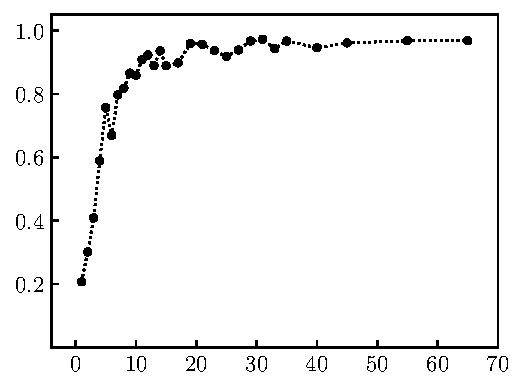
\includegraphics[scale=0.55]{albovo2024fig1a.pdf} &
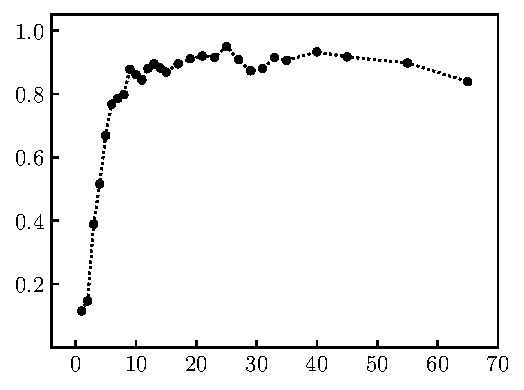
\includegraphics[scale=0.55]{albovo2024fig1b.pdf} &
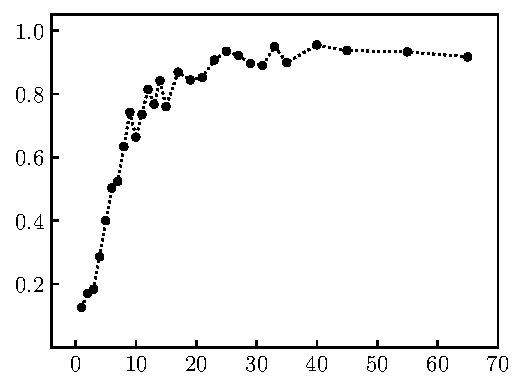
\includegraphics[scale=0.55]{albovo2024fig1c.pdf} \\
(a) measles & (b) mumps & (c) rubella
\end{tabular}
\end{center}
\caption{Observed proportion of seropositive for the three considered diseases.}
\label{fig1}
\end{figure}

\begin{figure}[ht!]
\begin{center}
\begin{tabular}{ccc}
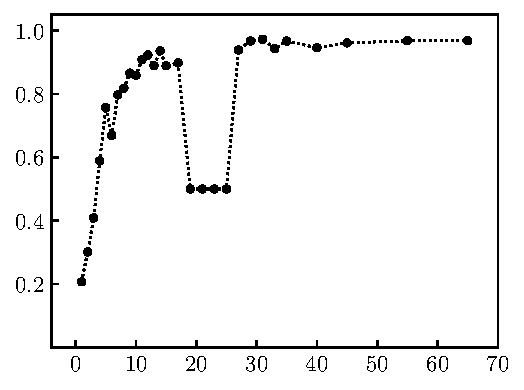
\includegraphics[scale=0.55]{albovo2024fig2a.pdf} &
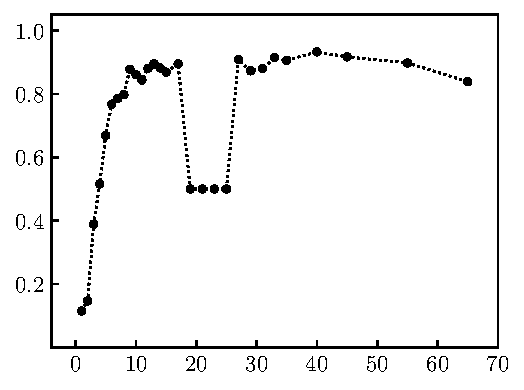
\includegraphics[scale=0.55]{albovo2024fig2b.pdf} &
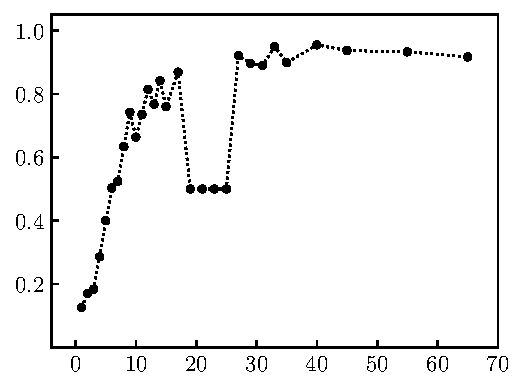
\includegraphics[scale=0.55]{albovo2024fig2c.pdf} \\
(a) measles & (b) mumps & (c) rubella
\end{tabular}
\end{center}
\caption{Observed proportion of seropositive for the three considered diseases after the inclusion of outliers.}
\label{fig2}
\end{figure}

We solved the OVO problem~\eqref{ovoprob} with $o \in \{0,1,\dots,10\}$. Table~\ref{tab2} and Figure~\ref{fig3} show the results. The table shows, for each value of $o$, the smallest value found for the OVO function (column $f(x^*)$) and, as a measure of Algorithm~\ref{sec:method}.1 performance, the number of iterations (column ``\#it''), the number of functional evaluations (column ``\#fcnt''), and the CPU time in seconds (column ``Time'') that were necessary to meet the stopping criterion. The figures in the table show that the smallest value found for the objective function of the OVO problem is on the order of $10^{-2}$ when $o \leq 3$ and drops by an order of magnitude when $o \geq 4$. This shows that this approach might be used to automatically detect the number of outliers contained in the data. In the figure, some of the curves appear overlapped, but as expected the models whose parameters were fitted considering $0 \leq o \leq 3$ fail to reproduce the observed data.

Figure~\ref{fig4} shows, on the left, the models adjusted when considering $o \in \{4,5,6\}$. It is not entirely clear that the model found by considering $o=4$ is ``the best''; and comparing the values of $f(x^*)$ obtained in the three cases does not help to decide, since it is natural that the more observations are left out, the better (smaller) is the value found. This suggests that, assuming model~\eqref{seropositives_model} is ``correct'', there are already outliers in the observed data available in~\cite{farrington}. Figure~\ref{fig4} shows on the right side the fitted models considering $o=10$. In these plots, the observations that the optimal solution of the OVO problem points out as outliers are highlighted in red. It is clear that choosing these observations manually would be practically impossible.

\begin{figure}[ht!]
\begin{center}
\begin{tabular}{cc}
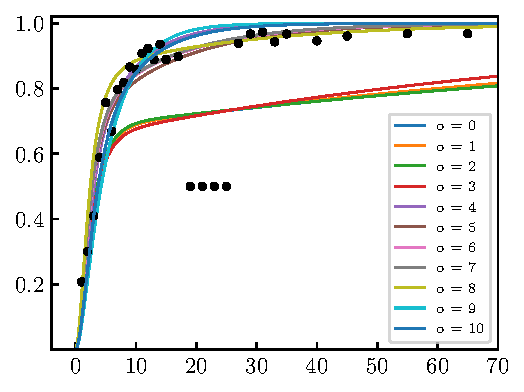
\includegraphics[scale=0.85]{albovo2024fig3a.pdf} &
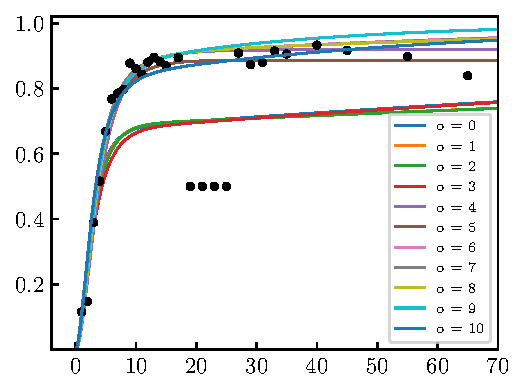
\includegraphics[scale=0.85]{albovo2024fig3b.pdf} \\
(a) measles & (b) mumps \\
\multicolumn{2}{c}{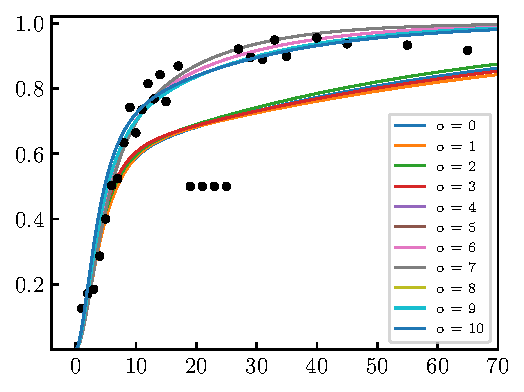
\includegraphics[scale=0.85]{albovo2024fig3c.pdf}} \\
\multicolumn{2}{c}{(c) rubella} \\
\end{tabular}
\end{center}
\caption{Models adjusted by solving the OVO problem of Section~\ref{numexp1} with $p=m-o$ and $o \in \{0,1,\dots,10\}$.}
\label{fig3}
\end{figure}

\begin{table}[ht!]
\begin{center}
\resizebox{\textwidth}{!}{\begin{tabular}{|c|cccc|cccc|cccc|}
\hline
\multirow{2}{*}{$o$} & 
\multicolumn{4}{c|}{measles} & 
\multicolumn{4}{c|}{mumps} & 
\multicolumn{4}{c|}{rubella}\\
\cline{2-13}
& $f(x^*)$ & \#it & \#fcnt & Time & $f(x^*)$ & \#it & \#fcnt & Time & $f(x^*)$ & \#it & \#fcnt & Time\\
\hline
\hline
  0 &  2.688E$-$02 &   8 &  40 &  3.463E$-$03 &  2.161E$-$02 &   9 &  28 &  2.811E$-$03 &  2.161E$-$02 &   7 &  33 &  2.102E$-$03 \\
  1 &  2.638E$-$02 &   5 &  19 &  1.735E$-$03 &  2.125E$-$02 &   5 &  12 &  1.963E$-$03 &  2.151E$-$02 &   5 &  27 &  1.397E$-$03 \\
  2 &  2.609E$-$02 &   5 &  19 &  1.874E$-$03 &  2.107E$-$02 &   4 &  11 &  1.578E$-$03 &  1.969E$-$02 &  23 &  56 &  3.256E$-$03 \\
  3 &  2.550E$-$02 &   8 &  30 &  3.086E$-$03 &  2.087E$-$02 &   4 &  13 &  2.114E$-$03 &  2.017E$-$02 &   7 &  17 &  1.478E$-$03 \\
  4 &  3.496E$-$03 &  16 &  34 &  1.997E$-$03 &  3.180E$-$03 &  10 &  34 &  3.162E$-$03 &  3.172E$-$03 &   4 &  21 &  2.127E$-$03 \\
  5 &  2.871E$-$03 &   8 &  15 &  2.500E$-$03 &  1.760E$-$03 &   6 &  18 &  1.295E$-$03 &  2.999E$-$03 &   4 &  11 &  1.782E$-$03 \\
  6 &  2.084E$-$03 &   3 &   7 &  1.165E$-$03 &  1.356E$-$03 &   5 &  12 &  2.235E$-$03 &  2.825E$-$03 &   4 &  11 &  1.818E$-$03 \\
  7 &  1.651E$-$03 &   7 &  12 &  1.483E$-$03 &  1.315E$-$03 &   5 &  10 &  1.830E$-$03 &  1.983E$-$03 &   3 &   9 &  1.053E$-$03 \\
  8 &  1.136E$-$03 &   6 &  12 &  2.211E$-$03 &  1.086E$-$03 &   6 &  13 &  2.614E$-$03 &  2.617E$-$03 &   4 &  11 &  1.127E$-$03 \\
  9 &  2.286E$-$03 &   3 &   4 &  9.820E$-$04 &  1.113E$-$03 &   4 &   8 &  1.928E$-$03 &  2.492E$-$03 &   4 &  20 &  1.419E$-$03 \\
 10 &  1.187E$-$03 &   2 &   3 &  9.740E$-$04 &  1.065E$-$03 &   4 &   9 &  1.877E$-$03 &  1.751E$-$03 &   5 &  12 &  1.809E$-$03 \\
\hline
\end{tabular}}
\end{center}
\caption{Details of applying Algorithm~\ref{sec:method}.1 for solving the OVO problem of Section~\ref{numexp1} with $p=m-o$ and $o \in \{0,1,\dots,10\}$.}
\label{tab2}
\end{table}

\begin{figure}[ht!]
\begin{center}
\begin{tabular}{cc}
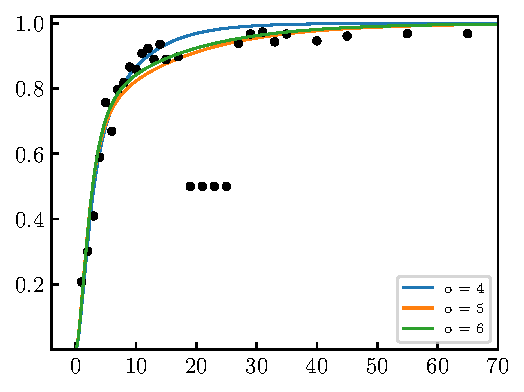
\includegraphics[scale=0.80]{albovo2024fig4a.pdf} &
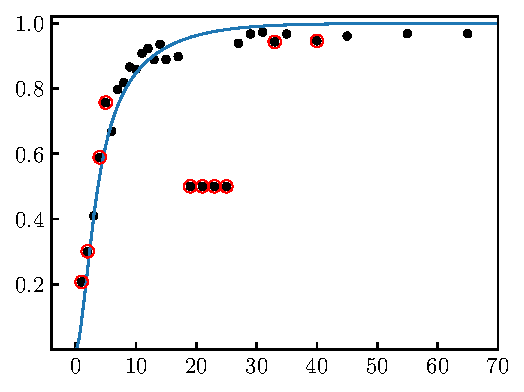
\includegraphics[scale=0.80]{albovo2024fig4d.pdf} \\
(a) measles & (d) measles \\
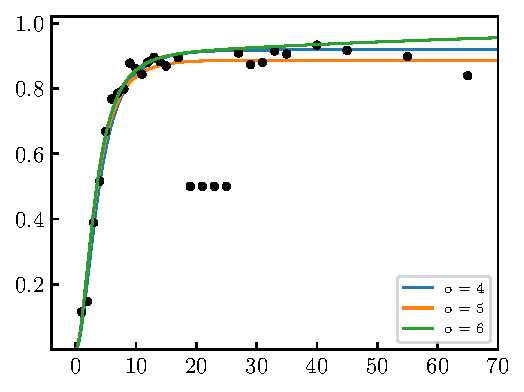
\includegraphics[scale=0.80]{albovo2024fig4b.pdf} &
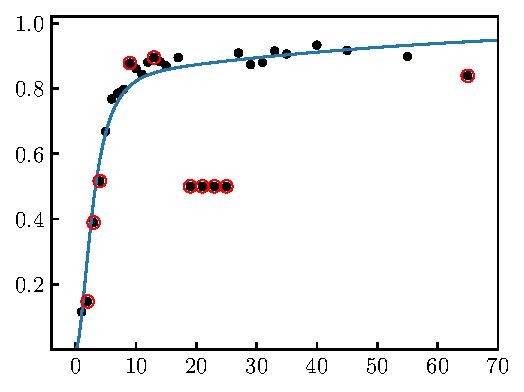
\includegraphics[scale=0.80]{albovo2024fig4e.pdf} \\
(b) mumps & (e) mumps \\
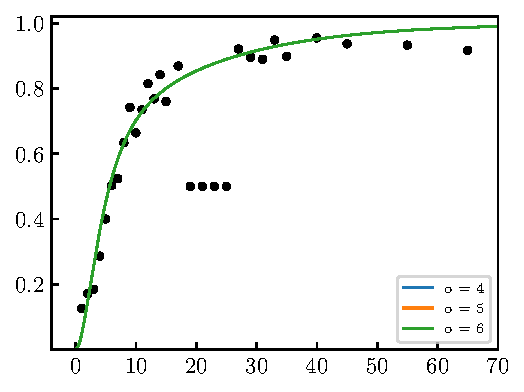
\includegraphics[scale=0.80]{albovo2024fig4c.pdf} &
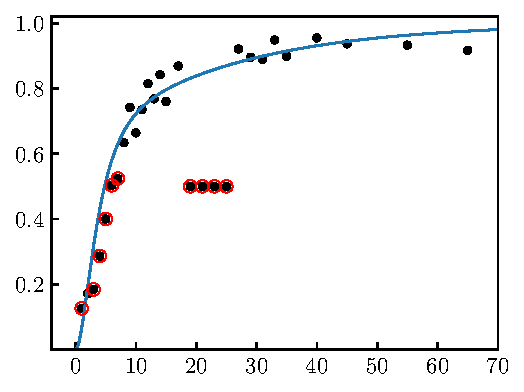
\includegraphics[scale=0.80]{albovo2024fig4f.pdf} \\
(c) rubella & (f) rubella \\
\end{tabular}
\end{center}
\caption{On the left side, the models fitted with $p=m-o$ and $o \in \{4,5,6\}$. On the right side, the models fitted with $o=10$, highlighting the observations that the optimal solution to the OVO problem points to as outliers.}
\label{fig4}
\end{figure}

\subsection{Osborne II function} \label{numexp2}

In the present section, following~\cite{yano2}, we consider a variation of problem Osborne II from~\cite{mgh}. The problem consists in finding parameters $x_1,\dots,x_{11}$ to fit the model
\[
y(t,x) = x_1 \exp(-t x_5) + x_2 \exp(-(t-x_9)^2 x_6) + x_3 \exp(-(t-x_{10})^2 x_7) + x_4 \exp(-(t-x_{11})^2 x_8)
\]
to data $(t_i,y_i)$ for $i=1,\dots,65$ reported in~\cite[p.25]{mgh}. The variation consists in introducing 13 additional data representing outliers. The outliers were taken from~\cite{yano2}. Considering the original data plus the 13 outliers, we arrive to $m=78$. There are no constraints in the unknown parameters and, therefore, $\Omega=\R^n$ in this case. As initial guess $x^0$, we considered the least squares solution using the data with the inclusion of outliers, namely, $x^0 \approx (1.312197, 0.367105, 0.551044, 0.642714, 0.596455, 2.306908, 0.365859, 8.197276$, $2.016720$, $4.339855, 5.686341)^T$. We solved the OVO problem~\eqref{ovoprob} with $o \in \{ 0, 1, \dots, 15\}$. Table~\ref{tab3} shows the results. The clear drop in the value of $f(x^*)$ when $o=13$ shows that the method correctly identified the number of outliers. The slightly increase in the value of $f(x^*)$ from $o=6$ to $o=7$, from $o=7$ to $o=8$, and from $o=13$ to $o=14$ shows that the method may be finding local non-global solutions. Anyway, it does not effect the identification of the correct number of outliers neither the adequate model fit for the case $o=13$.

Figure~\ref{fig5} illustrates the models found for the cases $o \in \{ 0, 3, 8, 13 \}$. It is clear that the cases with $o \neq 13$ are very poor due to the presence of the outliers, while the case $o=13$ corresponds to a model that correctly represents the real data. In~\cite{yano2}, a different problem is solved to fit the model: the function being minimized is the LOVO function defined as $f(x) = \sum_{j=1}^p f_{i_j}(x)$ instead of the OVO function defined as $f(x) = f_{i_p}(x)$ and considered in the present work. Moreover, since the problem is different, a different method is employed, for which the stopping criterion is not mentioned. Anyway, comparing Table~\ref{tab3} with~\cite[p.~18, Table~1]{yano2}, it is possible to see that both methods employ a similar number of iterations and function evaluations. Additionally, a comparison between Figure~\ref{fig5} and~\cite[p.~18, Figure~2]{yano2} shows that solutions found are qualitative equivalent.

\begin{table}[ht!]
\begin{center}
%\resizebox{\textwidth}{!}{
\begin{tabular}{|c|c|c|c|c|}
\hline
$o$ & $f(x^*)$ & \#it & \# fcnt & Time\\
\hline
\hline
   0 &  8.055e$-$02 &  85 &  139 &  3.561e$-$02 \\
   1 &  6.788e$-$02 &  17 &   44 &  5.022e$-$03 \\
   2 &  4.640e$-$02 &  30 &  100 &  1.441e$-$02 \\
   3 &  4.585e$-$02 &  28 &   82 &  1.543e$-$02 \\
   4 &  3.917e$-$02 &  13 &   43 &  8.359e$-$03 \\
   5 &  3.705e$-$02 &  18 &   58 &  1.114e$-$02 \\
   6 &  3.633e$-$02 &  30 &   44 &  1.360e$-$02 \\
   7 &  3.651e$-$02 &   7 &   18 &  5.089e$-$03 \\
   8 &  3.694e$-$02 &  10 &   31 &  4.082e$-$03 \\
   9 &  3.673e$-$02 &  28 &   37 &  8.291e$-$03 \\
  10 &  3.640e$-$02 &   5 &   12 &  2.610e$-$03 \\
  11 &  2.615e$-$02 &  12 &   38 &  3.815e$-$03 \\
  12 &  2.306e$-$02 &   7 &   27 &  2.659e$-$03 \\
  13 &  3.714e$-$03 &  26 &   62 &  1.269e$-$02 \\
  14 &  3.828e$-$03 &  22 &   48 &  1.406e$-$02 \\
  15 &  2.804e$-$03 &  35 &   69 &  2.797e$-$02 \\
\hline
\end{tabular}
\end{center}
\caption{Details of applying Algorithm~\ref{sec:method}.1 for solving the OVO problem of Section~\ref{numexp2} with $p=m-o$ and $o \in \{0, 1,\dots,15\}$.}
\label{tab3}
\end{table}

\begin{figure}[ht!]
\begin{center}
\begin{tabular}{cc}
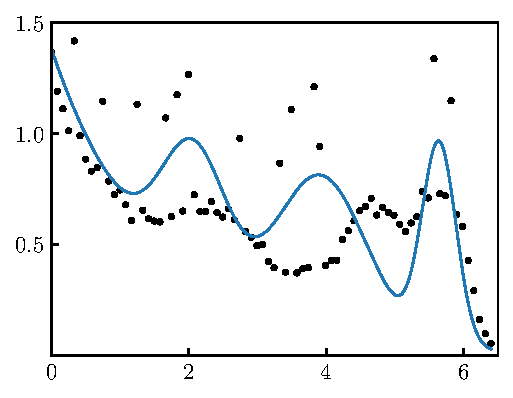
\includegraphics[scale=0.85]{albovo2024fig5a.pdf} &
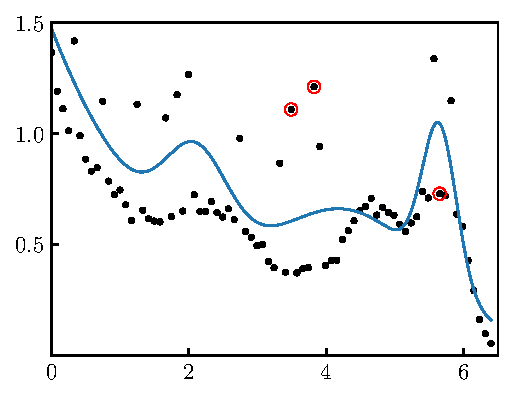
\includegraphics[scale=0.85]{albovo2024fig5b.pdf} \\
(a) $o=0$ & (b) $o=3$ \\
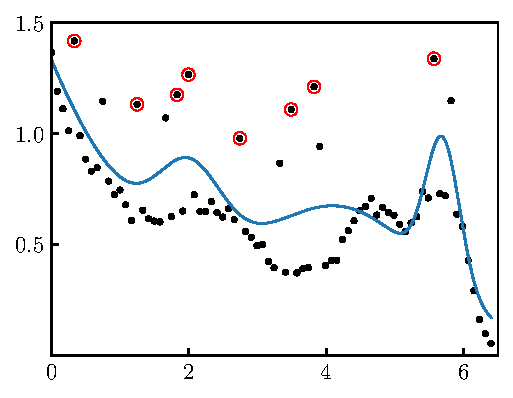
\includegraphics[scale=0.85]{albovo2024fig5c.pdf} &
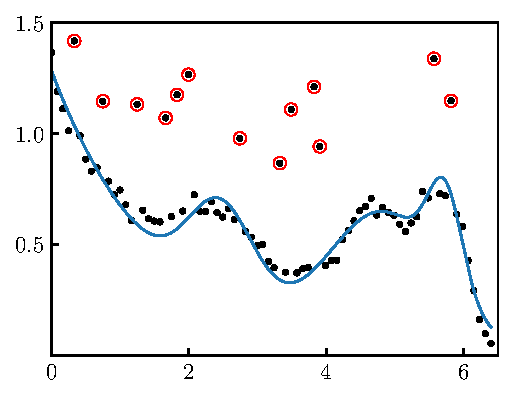
\includegraphics[scale=0.85]{albovo2024fig5d.pdf} \\
(c) $o=8$ & (d) $o=13$ \\
\end{tabular}
\end{center}
\caption{Models adjusted by solving the OVO problem of Section~\ref{numexp2} with $p=m-o$ and $o \in \{ 0, 3, 8, 13 \}$.}
\label{fig5}
\end{figure}

\subsection{Third degree polynomial in the canonical basis} \label{numexp3}  
In the present section, following~\cite{dunder1}, we consider the model
\[
y(t,x) = x_1 + x_2 t + x_3 t^2 + x_4 t^3,
\]
where $x_1, x_2, x_3, x_4$ are unknown parameters satisfying $-10 \leq x_i \leq 10$ for $i=1,\dots,4$. Therefore, we define $\Omega$ accordingly. A set of $m=47$ data $(t_i,y_i)$ containing 10 outliers was taken from~\cite{dunder1}. The least squares solution using the data with the inclusion of outliers is given by $\bar x \approx (6.460187,2.707182,-7.541815,2.160429)^T$. As the OVO problem may have many non-global local minimizers, in this experiment we considered 100 different starting points given by $x^0$ with components $x^0_i = \bar x_i + r | x^0_i |$, where $r \in [-0.5,0.5]$ is a random number with uniform distribution. For each considered value of $o \in \{0,\dots,12\}$, we report the best minimizer found. Table~\ref{tab4} shows the results while Figure~\ref{fig6} illustrates the solutions obtained for the cases $o \in \{ 0, 4, 8, 10 \}$. In the table, the sudden drop of $f(x^*)$ from the case $o=9$ to the case $o=10$ shows that the method is able to clearly detect the amount of outliers contained in the data. The table also shows that from case $o=0$ to case $o=10$ the value of $f(x^*)$ decreases monotonically, as expected. The cases $o=11$ and $o=12$ are not very relevant and the values of $f(x^*)$ are similar to the case $o=10$. But the fact that they are slightly larger than the value of case $o=10$ shows that the algorithm found local solutions of good quality but not corresponding to a global minimizer. Figure~\ref{fig6}(d) shows that, when the number of outliers is identified, the model fit is very good. Figures~\ref{fig6}(a-c) are interesting because they show the type of fit that is possible when the data are considered to contain fewer outliers than they actually do. 

In~\cite{dunder1}, a first-order method for the OVO problem was proposed. The proposed method is similar to the one presented in the present work. The main difference is that in subproblem~\eqref{covo-subpro}, instead of penalizing $\|x-\bar x\|^2$, a box constraint of the form $\|x-\bar x\|_{\infty} \leq \Delta$ is considered. This difference is what allows the method proposed in the present work to pose a worst-case analysis that provides an upper bound for the number of iterations and function evaluations that are necessary to find a solution with a prescribed accuracy. On the opposite side, the method proposed in~\cite{dunder1} presents a classical asymptotic convergence theory. If on the one hand the two methods have such a difference in their theoretical properties, it is not expected that they behave very differently in practice. This is exactly what Table~\ref{tab4} shows. In~\cite{dunder1} neither the stopping criterion nor the number of function evaluations is reported, but~\cite[p.~398, Table~2]{dunder1} shows a number of iterations compatible with (in fact, a slightly larger than) the number of iterations of our method, as shown in Table~\ref{tab4}.


\begin{table}[ht!]
\begin{center}
\begin{tabular}{|c|c|c|c|c|}
\hline
$o$ & $f(x^*)$ & \#it & \# fcnt & Time\\
\hline
\hline
 0 &  1.363e$+$01 &  27 &  105 &  1.483e$-$02 \\
 1 &  1.145e$+$01 &  37 &  170 &  3.047e$-$02 \\
 2 &  1.004e$+$01 &  40 &  194 &  1.381e$-$02 \\
 3 &  9.535e$+$00 &  39 &  190 &  2.557e$-$02 \\
 4 &  9.013e$+$00 &  40 &  164 &  3.945e$-$02 \\
 5 &  8.455e$+$00 &  38 &  170 &  2.586e$-$02 \\
 6 &  7.436e$+$00 &  44 &  225 &  2.646e$-$02 \\
 7 &  6.921e$+$00 &  38 &  206 &  2.109e$-$02 \\
 8 &  5.503e$+$00 &  43 &  210 &  2.453e$-$02 \\
 9 &  4.176e$+$00 &  25 &  117 &  2.020e$-$02 \\
10 &  3.120e$-$02 &  31 &  154 &  2.421e$-$02 \\
11 &  3.452e$-$02 &  28 &  145 &  1.852e$-$02 \\
12 &  3.228e$-$02 &  50 &  262 &  2.080e$-$02 \\
\hline
\end{tabular}
\end{center}
\caption{Details of applying Algorithm~\ref{sec:method}.1 for solving the OVO problem of Section~\ref{numexp3} with $p=m-o$ and $o \in \{0, 1,\dots,12\}$.}
\label{tab4}
\end{table}

\begin{figure}[ht!]
\begin{center}
\begin{tabular}{cc}
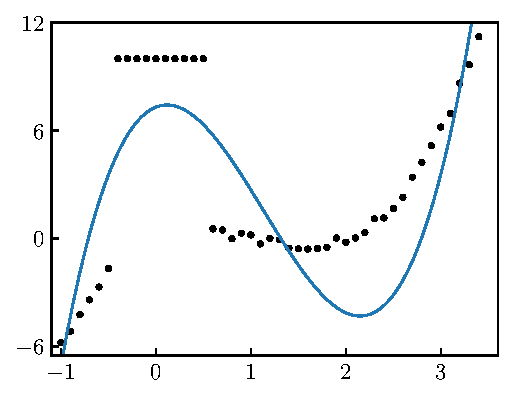
\includegraphics[scale=0.85]{albovo2024fig6a.pdf} &
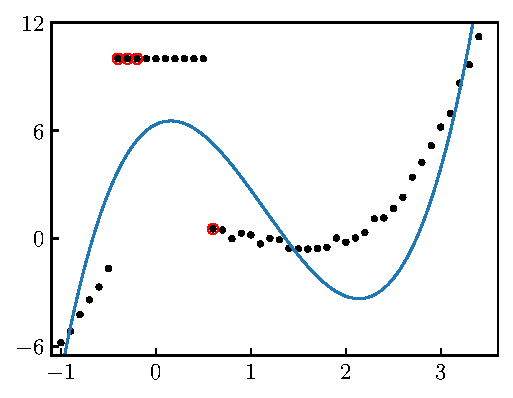
\includegraphics[scale=0.85]{albovo2024fig6b.pdf} \\
(a) $o=0$ & (b) $o=4$ \\
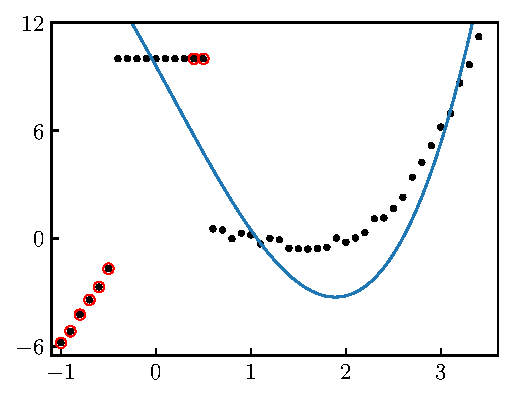
\includegraphics[scale=0.85]{albovo2024fig6c.pdf} &
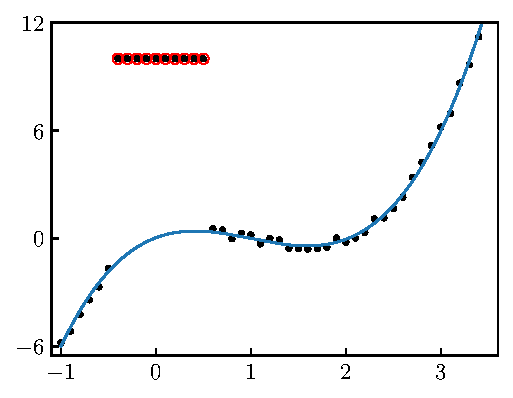
\includegraphics[scale=0.85]{albovo2024fig6d.pdf} \\
(c) $o=8$ & (d) $o=10$ \\
\end{tabular}
\end{center}
\caption{Models fitted solving the OVO problem of Section~\ref{numexp3} with $p=m-o$ and $o \in \{0, 4, 8, 10\}$.}
\label{fig6}
\end{figure}

We end this section by showing that the proposed method can be applied to problems with an increasing amount of data. For this purpose we consider problems with $m \in \{ 10^2, 10^3, \dots, 10^6 \}$ observations. Let $t_{\min}=-1$, $t_{\max}=3.5$, $t_i=t_{\min} + \left(\frac{i-1}{m-1}\right)(t_{\max}-t_{\min})$ for $i=1,\dots,m$, and $\tilde x = (0,2,-3,-1)^T$. Each $y_i$ is considered an outlier with probability 0.1. If the data is not an outlier, $y_i$ corresponds to $y(t_i,\tilde x)$ plus noise $r \in [-0.5,0.5]$. If the data is considered an outlier, it is larger than $y(t_i,\tilde x)$ with probability 0.8 and smaller with probability 0.2. If greater, it is a random value between $y(t_i,\tilde x)$ and 15. If less, it is a random value between $-6$ and $y(t_i,\tilde x)$. Figure~\ref{fig7} shows the data for the case $m=1{,}000$ as an example. This way of generating data is similar to the one used in~\cite{dunder1} to generate the problem with $m=47$ presented above. The figure shows that some of the data generated as outliers are identical to data generated as ``correct''. Therefore, discovering the exact number of generated outliers is impossible. Or, in other words, not all data generated as outliers are in fact outliers.

\begin{figure}[ht!]
\begin{center}
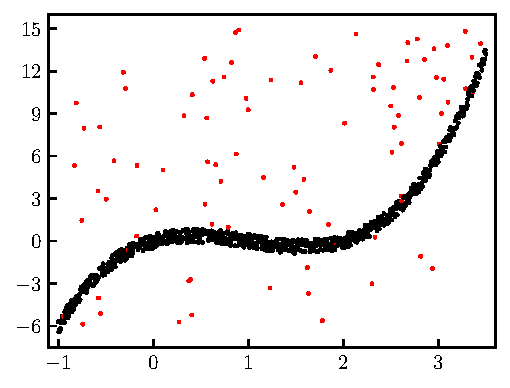
\includegraphics[scale=1.0]{albovo2024fig7.pdf}
\end{center}
\caption{Data with outliers for the case $m=1{,}000$. For those readers who are viewing the figure with colors, the black dots are the data generated as ``correct'' (contaminated with noise), while the red dots are the data generated as outliers.}
\label{fig7}
\end{figure}

For the case $m=100$, we solved OVO problems with $o$ varying from~5 to~15 in increments of~1. (The expected number of outliers is~10 in this case). For the case $m=1{,}000$, which has an expected number of outliers of~100, we vary $o$ from~50 to 150 in increments of~1. For the case $m=10{,}000$, we vary $o$ from 500 to $1{,}500$ in increments of~10. For the case $m=100{,}000$, we vary $o$ from $5{,}000$ to $15{,}000$ in increments of~100. For the case $m=1{,}000{,}000$, we vary $o$ from $50{,}000$ to $150{,}000$ in increments of~$1{,}000$. For each value of $o$, we solved the problem starting from 100 different starting points, as in the case with $m=47$ presented above. For each value of $m$, Figure~\ref{fig8} shows the value of $f(x^*)$ as a function of $o$ (for each $o$, the best value of the~100 runs is shown). The figure shows that in all cases there is a sharp drop of the value of $f(x^*)$ when an approximately correct number of outliers is considered. Note that the exact number of outliers is unknown because of the way they are generated and because when a data is generated as an outlier, it may in some cases look very similar to a real data. Moreover, not all values of $o$ are tested in the experiment. Even under these conditions, the figures show that the method succeeds perfectly well in identifying and disregarding outliers. In Table~\ref{tab5} we show, for each value of $m$, the amount $\bar o$ of data that were generated as outliers, and the smallest value of $o$ for which a value of $f(x^*)$ considered ``small'' is obtained (i.e.\ the first value of $o$ after the drop in the value of $f(x^*)$). For these selected cases, performance metrics of the method (number of iterations, number of function evaluations, and CPU time in seconds) are shown. The column showing the time per function evaluation suggests that the cost of the function evaluations increases linearly with the number of data $m$, although it includes a $m \log(m)$ ordering of the $f_i$ for $i=1,\dots,m$.

\begin{figure}[ht!]
\begin{center}
\begin{tabular}{cc}
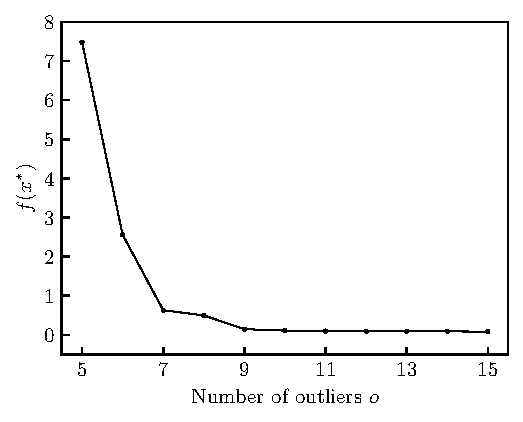
\includegraphics[scale=0.70]{albovo2024fig8a.pdf} &
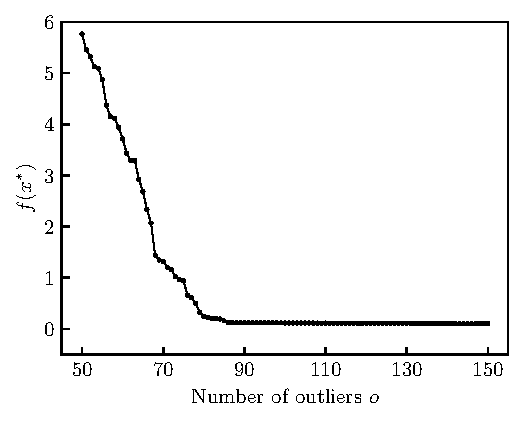
\includegraphics[scale=0.70]{albovo2024fig8b.pdf} \\
(a) $m=100$ & (b) $m=1{,}000$ \\
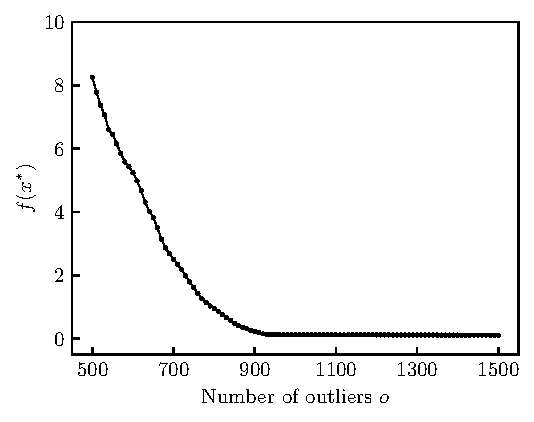
\includegraphics[scale=0.70]{albovo2024fig8c.pdf} &
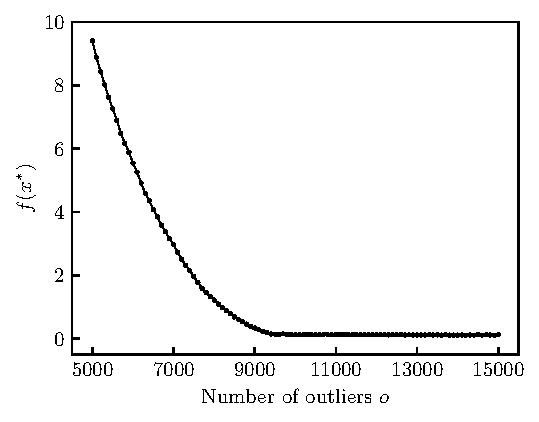
\includegraphics[scale=0.70]{albovo2024fig8d.pdf} \\
(a) $m=10{,}000$ & (b) $m=100{,}000$ \\
\multicolumn{2}{c}{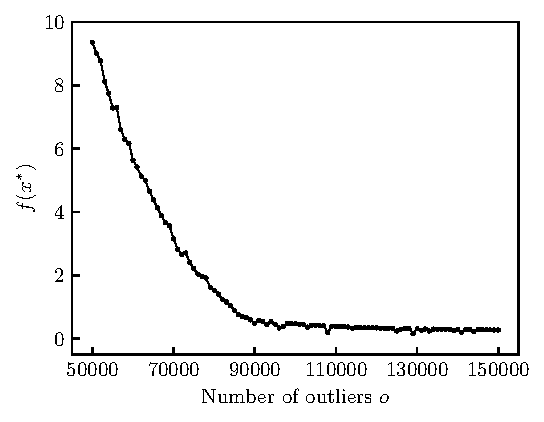
\includegraphics[scale=0.70]{albovo2024fig8e.pdf}} \\
\multicolumn{2}{c}{(c) $m=1{,}000{,}000$} \\
\end{tabular}
\end{center}
\caption{For each value of $o$ within a predefined interval, we solve an OVO problem with fixed~$o$ using 100 different starting points and keep the best $x^*$. These plots show $f(x^*)$ as a function of $o$. The graphs show that $f(x^*)$ decreases in an accentuated way up to a certain value of $o$ and, from that point on, it decreases very slowly. The smallest value of $o$ for which $f(x^*)$ decreases slowly is the value detected by the strategy as ``amount of outliers contained in the data''.}
\label{fig8}
\end{figure}

\begin{table}[ht!]
\begin{center}
\begin{tabular}{|c|c|c|c|c|c|c|c|c|}
\hline
$m$ & $\bar o$ & $o$ & $f(x^*)$ & \#it & \#fcnt & Time & Time / \#fcnt \\
\hline
\hline
          100 &     10 &     11 &  9.852E$-$02 &  65 &  467 &  2.486E$-$02 &  5.324E$-$05 \\
      1{,}000 &     92 &     85 &  1.567E$-$01 &  72 &  469 &  5.224E$-$02 &  1.114E$-$04 \\
     10{,}000 &    980 &    910 &  1.905E$-$01 &  38 &  224 &  1.511E$-$01 &  6.747E$-$04 \\
    100{,}000 &  10024 &   9300 &  1.887E$-$01 &  21 &   90 &  6.726E$-$01 &  7.473E$-$03 \\
1{,}000{,}000 & 100083 & 108000 &  1.863E$-$01 &   4 &   13 &  1.070E$+$00 &  8.233E$-$02 \\
\hline
\end{tabular}
\end{center}
\caption{Details of the performance of Algorithm~\ref{sec:method}.1 when solving OVO problems with increasing amount of data $m$.}
\label{tab5}
\end{table}

\section{Final remarks} \label{sec:conclu}

In this paper we introduced a method for the problem of minimizing the order-value function with box constraints. The method is of first order and uses quadratic regularization. As lines of future work we can mention the development of methods for problems with more general constraints and methods using higher order models. Generalized order-value functions are functions whose evaluation at a point $x$ of the domain depends on the order relation of the elements in a set of the form ${f_i(x)}_{i \in \mathcal{I}}$, where $\mathcal{I} \subset \N$ is a finite set of indices. Problems that include such functions in their definition, either in the objective function or in the constraints, are called generalized order-value optimization (GOVO) problems~\cite{mtop}. The problem considered in the present work belongs to this family of problems. Proposing methods with complexity results for other problems of the GOVO family is also a possible line of future work.\\

\noindent\textbf{Disclosure statement:} The authors report there are no competing interests to declare.

%\clearpage

\begin{thebibliography}{99}

\bibitem{abmsobso} R. Andreani, E. G. Birgin, J. M. Mart\'{\i}nez and M. L. Schuverdt, Augmented Lagrangian methods under the Constant Positive Linear Dependence constraint qualification, \textit{Mathematical Programming} 111, pp. 5--32, 2008.

\bibitem{abmstango} R. Andreani, E. G. Birgin, J. M. Mart\'{\i}nez and M. L. Schuverdt, On Augmented Lagrangian methods with general lower-level constraints, \textit{SIAM Journal on Optimization} 18, pp. 1286--1309, 2008.

\bibitem{dunder1} R. Andreani, C. Dunder and J. M. Mart\'{\i}nez, Order-Value Optimization: Formulation and solution by means of a primal Cauchy method, \textit{Mathematical Methods of Operations Research} 58, pp. 387--399, 2003.

\bibitem{dunder2} R. Andreani, C. Dunder and J. M. Mart\'{\i}nez, Nonlinear-programming reformulation of the order-value optimization problem, \textit{Mathematical Methods of Operations Research} 61, pp. 365--384, 2005.

\bibitem{yano1} R. Andreani, J. M. Mart\'{\i}nez, M. Salvatierra, and F. S. Yano, Quasi-Newton methods for Order-Value Optimization and Value-at-Risk calculations, \textit{Pacific Journal of Optimization} 2, pp. 11--33, 2006.

\bibitem{yano2} R. Andreani, J. M. Mart\'{\i}nez, L. Mart\'{\i}nez, and F. S. Yano, Low order-value optimization and applications, \textit{Journal of Global Optimization} 43, pp. 1--22, 2009.

\bibitem{salva} R. Andreani, J. M. Mart\'{\i}nez, M. Salvatierra, and F. S. Yano, Global order-value optimization by means of a multistart harmonic oscillator tunneling strategy, in \textit{Global Optimization: From Theory to Implementation}, L. Liberti and N. Maculan (eds.), Springer, Boston, MA, 2006, pp. 379--404.

\bibitem{bgms} E. G. Birgin, J. L. Gardenghi, J. M. Mart\'{\i}nez, and S. A. Santos, On the use of third-order models with fourth-order regularization for unconstrained optimization, \textit{Optimization Letters} 14, pp. 815--838, 2020.

\bibitem{bgmst2} E. G. Birgin, J. L. Gardenghi, J. M. Mart\'{\i}nez, S. A. Santos, and Ph. L. Toint, Evaluation complexity for nonlinear constrained optimization using unscaled KKT conditions and high-order models, \textit{SIAM Journal on Optimization} 26, pp. 951--967, 2016.

\bibitem{bgmst1} E. G. Birgin, J. L. Gardenghi, J. M. Mart\'{\i}nez, S. A. Santos, and Ph. L. Toint, Worst-case evaluation complexity for unconstrained nonlinear optimization using high-order regularized models, \textit{Mathematical Programming} 163, pp. 359--368, 2017.

\bibitem{bmbook} E. G. Birgin and J. M. Mart\'{\i}nez, \textit{Practical Augmented Lagrangian Methods for Constrained Optimization}, Society for Industrial and Applied Mathematics, Philadelphia, 2014.

\bibitem{bmcomper} E. G. Birgin and J. M. Mart\'{\i}nez, Complexity and performance of an Augmented Lagrangian algorithm, \textit{Optimization Methods and Software} 35, pp. 885--920, 2020.

\bibitem{cogtbook} C. Cartis, N. I. M. Gould, and Ph. L. Toint, \textit{Evaluation Complexity of Algorithms for Nonconvex Optimization: Theory, Computation, and Perspectives}, SIAM, Philadelphia, PA, 2022.

\bibitem{farrington} C. P. Farrington, Modelling forces of infection for measles, mumps and rubella, \textit{Statistics in Medicine} 9, pp. 953--967, 1990.

\bibitem{gauvin} J. Gauvin, A necessary and sufficient regularity condition to have bounded multipliers in nonconvex programming, \textit{Mathematical Programming} 12, pp. 136--138.
  
\bibitem{jorion} P. Jorion, \textit{Value at {R}isk: {T}he new benchmark for managing financial risk}, 3rd. ed., McGraw-Hill, 2009.

\bibitem{mtop} J. M. Mart\'{\i}nez, Generalized Order-Value Optimization, \textit{TOP} 20, pp. 75--98, 2012.

\bibitem{mgh} J. J. Mor\'e, B. S. Garbow, and K. E. Hillstrom, Testing unconstrained optimization software, \textit{ACM Transactions on Mathematical Software} 7, pp. 17--41, 1981.
  
\bibitem{nesterov} Y. Nesterov and B. T. Polyak, Cubic regularization of Newton method and its global performance, \textit{Mathematical Programming} 108, 177--205, 2006.

\bibitem{jiang} Z. Jiang, Q. Hu, and X. Zheng, Optimality condition and complexity of order-value optimization problems and low order-value optimization problems, \textit{Journal of Global Optimization} 69, pp. 511--523, 2017.
    
\end{thebibliography}

\end{document}
